\documentclass[a4paper]{book}
\usepackage{a4wide}
\usepackage{makeidx}
\usepackage{fancyhdr}
\usepackage{graphicx}
\usepackage{multicol}
\usepackage{float}
\usepackage{textcomp}
\usepackage{alltt}
\usepackage{doxygen}
\makeindex
\setcounter{tocdepth}{1}
\renewcommand{\footrulewidth}{0.4pt}
\begin{document}
\begin{titlepage}
\vspace*{7cm}
\begin{center}
{\Large CVRP-TW Reference Manual\\[1ex]\large 1.0 }\\
\vspace*{1cm}
{\large Generated by Doxygen 1.4.7}\\
\vspace*{0.5cm}
{\small Fri Dec 7 16:57:19 2007}\\
\end{center}
\end{titlepage}
\clearemptydoublepage
\pagenumbering{roman}
\tableofcontents
\clearemptydoublepage
\pagenumbering{arabic}
\chapter{Welcome to PARADISEO - CVRP-TW contribution }
\label{index}\section{Introduction}\label{main_Introduction}
The capacitated vehicle routing problem with time windows or CVRP-TW is a combinatorial optimization problem seeking to service a number of customers with a fleet of vehicles where the vehicles have a mimited capacity and the delivery locations have time windows within which the deliveries (or visits) must be made. Often the context is that of delivering goods located at a central depot to customers who have placed orders for such goods. Implicit is the goal of minimizing the cost of distributing the goods. Finding the global minimum for the cost function, except for the smallest instances, is computationally complex.\section{AUTHORS}\label{main_authors}
\begin{TabularC}{3}
\hline
Dolphin project-team INRIA Futurs, 2007. &Antonio La\-Torre atorre[at]fi.upm.es &Thomas Legrand paradiseo-help[at]lists.gforge.inria.fr  \\\hline
\end{TabularC}
\section{LICENSE}\label{main_LICENSE}
This software is governed by the Ce\-CILL license under French law and abiding by the rules of distribution of free software. You can use, modify and/ or redistribute the software under the terms of the Ce\-CILL license as circulated by CEA, CNRS and INRIA at the following URL \char`\"{}http://www.cecill.info\char`\"{}.

As a counterpart to the access to the source code and rights to copy, modify and redistribute granted by the license, users are provided only with a limited warranty and the software's author, the holder of the economic rights, and the successive licensors have only limited liability.

In this respect, the user's attention is drawn to the risks associated with loading, using, modifying and/or developing or reproducing the software by the user in light of its specific status of free software, that may mean that it is complicated to manipulate, and that also therefore means that it is reserved for developers and experienced professionals having in-depth computer knowledge. Users are therefore encouraged to load and test the software's suitability as regards their requirements in conditions enabling the security of their systems and/or data to be ensured and, more generally, to use and operate it in the same conditions as regards security. The fact that you are presently reading this means that you have had knowledge of the Ce\-CILL license and that you accept its terms.

Paradis\-EO Web\-Site : \tt{http://paradiseo.gforge.inria.fr} Contact: \tt{paradiseo-help@lists.gforge.inria.fr}\section{Home Page}\label{main_Paradiseo}
{\tt http://paradiseo.gforge.inria.fr} 
\chapter{CVRP-TW Namespace Index}
\section{Paradis\-EO-PEOMoving\-Objects Namespace List}
Here is a list of all documented namespaces with brief descriptions:\begin{CompactList}
\item\contentsline{section}{\hyperlink{namespacepeo}{peo} }{\pageref{namespacepeo}}{}
\end{CompactList}

\chapter{CVRP-TW Hierarchical Index}
\section{Paradis\-EO-MO-Moving\-Objects Class Hierarchy}
This inheritance list is sorted roughly, but not completely, alphabetically:\begin{CompactList}
\item \contentsline{section}{mo\-Algo$<$ EOT $>$}{\pageref{classmo_algo}}{}
\item \contentsline{section}{mo\-Aspir\-Crit$<$ M $>$}{\pageref{classmo_aspir_crit}}{}
\begin{CompactList}
\item \contentsline{section}{mo\-Impr\-Best\-Fit\-Aspir\-Crit$<$ M $>$}{\pageref{classmo_impr_best_fit_aspir_crit}}{}
\item \contentsline{section}{mo\-No\-Aspir\-Crit$<$ M $>$}{\pageref{classmo_no_aspir_crit}}{}
\end{CompactList}
\item \contentsline{section}{mo\-Comparator$<$ EOT $>$}{\pageref{classmo_comparator}}{}
\begin{CompactList}
\item \contentsline{section}{mo\-Fit\-Comparator$<$ EOT $>$}{\pageref{classmo_fit_comparator}}{}
\end{CompactList}
\item \contentsline{section}{mo\-Cooling\-Schedule}{\pageref{classmo_cooling_schedule}}{}
\begin{CompactList}
\item \contentsline{section}{mo\-Exponential\-Cooling\-Schedule}{\pageref{classmo_exponential_cooling_schedule}}{}
\item \contentsline{section}{mo\-Linear\-Cooling\-Schedule}{\pageref{classmo_linear_cooling_schedule}}{}
\end{CompactList}
\item \contentsline{section}{mo\-HC$<$ M $>$}{\pageref{classmo_h_c}}{}
\item \contentsline{section}{mo\-ILS$<$ M $>$}{\pageref{classmo_i_l_s}}{}
\item \contentsline{section}{mo\-LSCheck\-Point$<$ M $>$}{\pageref{classmo_l_s_check_point}}{}
\item \contentsline{section}{mo\-Move$<$ EOT $>$}{\pageref{classmo_move}}{}
\item \contentsline{section}{mo\-Move\-Expl$<$ M $>$}{\pageref{classmo_move_expl}}{}
\begin{CompactList}
\item \contentsline{section}{mo\-Move\-Loop\-Expl$<$ M $>$}{\pageref{classmo_move_loop_expl}}{}
\begin{CompactList}
\item \contentsline{section}{mo\-HCMove\-Loop\-Expl$<$ M $>$}{\pageref{classmo_h_c_move_loop_expl}}{}
\item \contentsline{section}{mo\-TSMove\-Loop\-Expl$<$ M $>$}{\pageref{classmo_t_s_move_loop_expl}}{}
\end{CompactList}
\end{CompactList}
\item \contentsline{section}{mo\-Move\-Incr\-Eval$<$ M $>$}{\pageref{classmo_move_incr_eval}}{}
\item \contentsline{section}{mo\-Move\-Init$<$ M $>$}{\pageref{classmo_move_init}}{}
\item \contentsline{section}{mo\-Move\-Select$<$ M $>$}{\pageref{classmo_move_select}}{}
\begin{CompactList}
\item \contentsline{section}{mo\-Best\-Impr\-Select$<$ M $>$}{\pageref{classmo_best_impr_select}}{}
\item \contentsline{section}{mo\-First\-Impr\-Select$<$ M $>$}{\pageref{classmo_first_impr_select}}{}
\item \contentsline{section}{mo\-Rand\-Impr\-Select$<$ M $>$}{\pageref{classmo_rand_impr_select}}{}
\end{CompactList}
\item \contentsline{section}{mo\-Next\-Move$<$ M $>$}{\pageref{classmo_next_move}}{}
\begin{CompactList}
\item \contentsline{section}{mo\-It\-Rand\-Next\-Move$<$ M $>$}{\pageref{classmo_it_rand_next_move}}{}
\end{CompactList}
\item \contentsline{section}{mo\-Rand\-Move$<$ M $>$}{\pageref{classmo_rand_move}}{}
\item \contentsline{section}{mo\-SA$<$ M $>$}{\pageref{classmo_s_a}}{}
\item \contentsline{section}{mo\-Sol\-Continue$<$ EOT $>$}{\pageref{classmo_sol_continue}}{}
\begin{CompactList}
\item \contentsline{section}{mo\-Fit\-Sol\-Continue$<$ EOT $>$}{\pageref{classmo_fit_sol_continue}}{}
\item \contentsline{section}{mo\-Gen\-Sol\-Continue$<$ EOT $>$}{\pageref{classmo_gen_sol_continue}}{}
\item \contentsline{section}{mo\-No\-Fit\-Impr\-Sol\-Continue$<$ EOT $>$}{\pageref{classmo_no_fit_impr_sol_continue}}{}
\item \contentsline{section}{mo\-Steady\-Fit\-Sol\-Continue$<$ EOT $>$}{\pageref{classmo_steady_fit_sol_continue}}{}
\end{CompactList}
\item \contentsline{section}{mo\-Tabu\-List$<$ M $>$}{\pageref{classmo_tabu_list}}{}
\begin{CompactList}
\item \contentsline{section}{mo\-Simple\-Move\-Tabu\-List$<$ M $>$}{\pageref{classmo_simple_move_tabu_list}}{}
\item \contentsline{section}{mo\-Simple\-Solution\-Tabu\-List$<$ M $>$}{\pageref{classmo_simple_solution_tabu_list}}{}
\end{CompactList}
\item \contentsline{section}{mo\-TS$<$ M $>$}{\pageref{classmo_t_s}}{}
\end{CompactList}

\chapter{CVRP-TW Class Index}
\section{Paradis\-EO-PEO-Parallelanddistributed\-Evolving\-Objects Class List}
Here are the classes, structs, unions and interfaces with brief descriptions:\begin{CompactList}
\item\contentsline{section}{\hyperlink{structAlgorithm}{Algorithm} }{\pageref{structAlgorithm}}{}
\item\contentsline{section}{\hyperlink{classCitySwap}{City\-Swap} (Its swaps two vertices randomly choosen )}{\pageref{classCitySwap}}{}
\item\contentsline{section}{\hyperlink{classCommunicable}{Communicable} }{\pageref{classCommunicable}}{}
\item\contentsline{section}{\hyperlink{classCommunicator}{Communicator} }{\pageref{classCommunicator}}{}
\item\contentsline{section}{\hyperlink{classCompleteTopology}{Complete\-Topology} }{\pageref{classCompleteTopology}}{}
\item\contentsline{section}{\hyperlink{classcontinuator}{continuator} (Abstract class for a continuator within the exchange of data by migration )}{\pageref{classcontinuator}}{}
\item\contentsline{section}{\hyperlink{classCooperative}{Cooperative} }{\pageref{classCooperative}}{}
\item\contentsline{section}{\hyperlink{classDisplayBestRoute}{Display\-Best\-Route} }{\pageref{classDisplayBestRoute}}{}
\item\contentsline{section}{\hyperlink{classEdgeXover}{Edge\-Xover} (Edge Crossover )}{\pageref{classEdgeXover}}{}
\item\contentsline{section}{\hyperlink{classeoContinuator}{eo\-Continuator$<$ EOT $>$} (Specific class for a continuator within the exchange of migration of a population )}{\pageref{classeoContinuator}}{}
\item\contentsline{section}{\hyperlink{classeoReplace}{eo\-Replace$<$ EOT, TYPE $>$} (Specific class for a replacement within the exchange of migration of a population )}{\pageref{classeoReplace}}{}
\item\contentsline{section}{\hyperlink{classeoSelector}{eo\-Selector$<$ EOT, TYPE $>$} (Specific class for a selector within the exchange of migration of a population )}{\pageref{classeoSelector}}{}
\item\contentsline{section}{\hyperlink{classeoSyncContinue}{eo\-Sync\-Continue} (Class for a continuator within the exchange of data by synchrone migration )}{\pageref{classeoSyncContinue}}{}
\item\contentsline{section}{\hyperlink{classMergeRouteEval}{Merge\-Route\-Eval} }{\pageref{classMergeRouteEval}}{}
\item\contentsline{section}{\hyperlink{classMPIThreadedEnv}{MPIThreaded\-Env} }{\pageref{classMPIThreadedEnv}}{}
\item\contentsline{section}{\hyperlink{classOrderXover}{Order\-Xover} (Order Crossover )}{\pageref{classOrderXover}}{}
\item\contentsline{section}{\hyperlink{classPartialMappedXover}{Partial\-Mapped\-Xover} (Partial Mapped Crossover )}{\pageref{classPartialMappedXover}}{}
\item\contentsline{section}{\hyperlink{classPartRouteEval}{Part\-Route\-Eval} (Route Evaluator )}{\pageref{classPartRouteEval}}{}
\item\contentsline{section}{\hyperlink{classpeoAggEvalFunc}{peo\-Agg\-Eval\-Func$<$ EOT $>$} (The \hyperlink{classpeoAggEvalFunc}{peo\-Agg\-Eval\-Func} class offers only the interface for creating aggregate evaluation functions - there are no direct internal functions provided )}{\pageref{classpeoAggEvalFunc}}{}
\item\contentsline{section}{\hyperlink{classpeoAsyncIslandMig}{peo\-Async\-Island\-Mig$<$ TYPESELECT, TYPEREPLACE $>$} (Specific class for a asynchronous migration )}{\pageref{classpeoAsyncIslandMig}}{}
\item\contentsline{section}{\hyperlink{structpeoEvalFunc}{peo\-Eval\-Func$<$ EOT, Fit\-T, Function\-Arg $>$} (Specific class for evaluation )}{\pageref{structpeoEvalFunc}}{}
\item\contentsline{section}{\hyperlink{classpeoGlobalBestVelocity}{peo\-Global\-Best\-Velocity$<$ POT $>$} (Specific class for a replacement thanks to the velocity migration of a population of a PSO )}{\pageref{classpeoGlobalBestVelocity}}{}
\item\contentsline{section}{\hyperlink{classpeoMultiStart}{peo\-Multi\-Start$<$ Entity\-Type $>$} (Class allowing the launch of several algorithms )}{\pageref{classpeoMultiStart}}{}
\item\contentsline{section}{\hyperlink{structpeoMultiStart_1_1AbstractAggregationAlgorithm}{peo\-Multi\-Start$<$ Entity\-Type $>$::Abstract\-Aggregation\-Algorithm} }{\pageref{structpeoMultiStart_1_1AbstractAggregationAlgorithm}}{}
\item\contentsline{section}{\hyperlink{structpeoMultiStart_1_1AbstractAlgorithm}{peo\-Multi\-Start$<$ Entity\-Type $>$::Abstract\-Algorithm} }{\pageref{structpeoMultiStart_1_1AbstractAlgorithm}}{}
\item\contentsline{section}{\hyperlink{structpeoMultiStart_1_1AbstractDataType}{peo\-Multi\-Start$<$ Entity\-Type $>$::Abstract\-Data\-Type} }{\pageref{structpeoMultiStart_1_1AbstractDataType}}{}
\item\contentsline{section}{\hyperlink{structpeoMultiStart_1_1AggregationAlgorithm}{peo\-Multi\-Start$<$ Entity\-Type $>$::Aggregation\-Algorithm$<$ Aggregation\-Algorithm\-Type $>$} }{\pageref{structpeoMultiStart_1_1AggregationAlgorithm}}{}
\item\contentsline{section}{\hyperlink{structpeoMultiStart_1_1Algorithm}{peo\-Multi\-Start$<$ Entity\-Type $>$::Algorithm$<$ Algorithm\-Type $>$} }{\pageref{structpeoMultiStart_1_1Algorithm}}{}
\item\contentsline{section}{\hyperlink{structpeoMultiStart_1_1DataType}{peo\-Multi\-Start$<$ Entity\-Type $>$::Data\-Type$<$ Type $>$} }{\pageref{structpeoMultiStart_1_1DataType}}{}
\item\contentsline{section}{\hyperlink{structpeoMultiStart_1_1FunctionAlgorithm}{peo\-Multi\-Start$<$ Entity\-Type $>$::Function\-Algorithm$<$ Algorithm\-Return\-Type, Algorithm\-Data\-Type $>$} }{\pageref{structpeoMultiStart_1_1FunctionAlgorithm}}{}
\item\contentsline{section}{\hyperlink{structpeoMultiStart_1_1NoAggregationFunction}{peo\-Multi\-Start$<$ Entity\-Type $>$::No\-Aggregation\-Function} }{\pageref{structpeoMultiStart_1_1NoAggregationFunction}}{}
\item\contentsline{section}{\hyperlink{classpeoNoAggEvalFunc}{peo\-No\-Agg\-Eval\-Func$<$ EOT $>$} (The \hyperlink{classpeoNoAggEvalFunc}{peo\-No\-Agg\-Eval\-Func} class does nothing more than an association between a fitness value and a specified individual )}{\pageref{classpeoNoAggEvalFunc}}{}
\item\contentsline{section}{\hyperlink{classpeoPopEval}{peo\-Pop\-Eval$<$ EOT $>$} (Parallel evaluation functor wrapper )}{\pageref{classpeoPopEval}}{}
\item\contentsline{section}{\hyperlink{classpeoPSOSelect}{peo\-PSOSelect$<$ POT $>$} (Specific class for a selection of a population of a PSO )}{\pageref{classpeoPSOSelect}}{}
\item\contentsline{section}{\hyperlink{classpeoSyncIslandMig}{peo\-Sync\-Island\-Mig$<$ TYPESELECT, TYPEREPLACE $>$} (Specific class for a synchronous migration )}{\pageref{classpeoSyncIslandMig}}{}
\item\contentsline{section}{\hyperlink{classpeoTransform}{peo\-Transform$<$ EOT $>$} (Class for a parallel transform )}{\pageref{classpeoTransform}}{}
\item\contentsline{section}{\hyperlink{classpeoWorstPositionReplacement}{peo\-Worst\-Position\-Replacement$<$ POT $>$} (Specific class for a replacement of a population of a PSO )}{\pageref{classpeoWorstPositionReplacement}}{}
\item\contentsline{section}{\hyperlink{classpeoWrapper}{peo\-Wrapper} (Specific class for wrapping )}{\pageref{classpeoWrapper}}{}
\item\contentsline{section}{\hyperlink{structpeoWrapper_1_1AbstractAlgorithm}{peo\-Wrapper::Abstract\-Algorithm} }{\pageref{structpeoWrapper_1_1AbstractAlgorithm}}{}
\item\contentsline{section}{\hyperlink{structpeoWrapper_1_1Algorithm}{peo\-Wrapper::Algorithm$<$ Algorithm\-Type, Algorithm\-Data\-Type $>$} }{\pageref{structpeoWrapper_1_1Algorithm}}{}
\item\contentsline{section}{\hyperlink{structpeoWrapper_1_1Algorithm_3_01AlgorithmType_00_01void_01_4}{peo\-Wrapper::Algorithm$<$ Algorithm\-Type, void $>$} }{\pageref{structpeoWrapper_1_1Algorithm_3_01AlgorithmType_00_01void_01_4}}{}
\item\contentsline{section}{\hyperlink{structpeoWrapper_1_1FunctionAlgorithm}{peo\-Wrapper::Function\-Algorithm$<$ Algorithm\-Return\-Type, Algorithm\-Data\-Type $>$} }{\pageref{structpeoWrapper_1_1FunctionAlgorithm}}{}
\item\contentsline{section}{\hyperlink{structpeoWrapper_1_1FunctionAlgorithm_3_01AlgorithmReturnType_00_01void_01_4}{peo\-Wrapper::Function\-Algorithm$<$ Algorithm\-Return\-Type, void $>$} }{\pageref{structpeoWrapper_1_1FunctionAlgorithm_3_01AlgorithmReturnType_00_01void_01_4}}{}
\item\contentsline{section}{\hyperlink{classRandomTopology}{Random\-Topology} }{\pageref{classRandomTopology}}{}
\item\contentsline{section}{\hyperlink{classReactiveThread}{Reactive\-Thread} }{\pageref{classReactiveThread}}{}
\item\contentsline{section}{\hyperlink{classreplacement}{replacement$<$ TYPE $>$} (Abstract class for a replacement within the exchange of data by migration )}{\pageref{classreplacement}}{}
\item\contentsline{section}{\hyperlink{classRingTopology}{Ring\-Topology} }{\pageref{classRingTopology}}{}
\item\contentsline{section}{\hyperlink{classRouteEval}{Route\-Eval} }{\pageref{classRouteEval}}{}
\item\contentsline{section}{\hyperlink{classRouteInit}{Route\-Init} }{\pageref{classRouteInit}}{}
\item\contentsline{section}{\hyperlink{classRunner}{Runner} }{\pageref{classRunner}}{}
\item\contentsline{section}{\hyperlink{classselector}{selector$<$ TYPE $>$} (Abstract class for a selector within the exchange of data by migration )}{\pageref{classselector}}{}
\item\contentsline{section}{\hyperlink{structSEND__REQUEST}{SEND\_\-REQUEST} }{\pageref{structSEND__REQUEST}}{}
\item\contentsline{section}{\hyperlink{classService}{Service} }{\pageref{classService}}{}
\item\contentsline{section}{\hyperlink{classStarTopology}{Star\-Topology} }{\pageref{classStarTopology}}{}
\item\contentsline{section}{\hyperlink{structSyncCompare}{Sync\-Compare} }{\pageref{structSyncCompare}}{}
\item\contentsline{section}{\hyperlink{structSyncEntry}{Sync\-Entry} }{\pageref{structSyncEntry}}{}
\item\contentsline{section}{\hyperlink{classThread}{Thread} }{\pageref{classThread}}{}
\item\contentsline{section}{\hyperlink{classTopology}{Topology} }{\pageref{classTopology}}{}
\item\contentsline{section}{\hyperlink{classTwoOpt}{Two\-Opt} }{\pageref{classTwoOpt}}{}
\item\contentsline{section}{\hyperlink{classTwoOptIncrEval}{Two\-Opt\-Incr\-Eval} }{\pageref{classTwoOptIncrEval}}{}
\item\contentsline{section}{\hyperlink{classTwoOptInit}{Two\-Opt\-Init} }{\pageref{classTwoOptInit}}{}
\item\contentsline{section}{\hyperlink{classTwoOptNext}{Two\-Opt\-Next} }{\pageref{classTwoOptNext}}{}
\item\contentsline{section}{\hyperlink{classTwoOptRand}{Two\-Opt\-Rand} }{\pageref{classTwoOptRand}}{}
\item\contentsline{section}{\hyperlink{classWorker}{Worker} }{\pageref{classWorker}}{}
\end{CompactList}

\chapter{CVRP-TW Namespace Documentation}
\section{eo\-VRPUtils Namespace Reference}
\label{namespaceeo_v_r_p_utils}\index{eoVRPUtils@{eoVRPUtils}}
A set of structures and utility functions for the VRP-TW problem.  


\subsection*{Classes}
\begin{CompactItemize}
\item 
struct \bf{Client\-Data}
\begin{CompactList}\small\item\em Information regarding each client in the dataset. \item\end{CompactList}\end{CompactItemize}
\subsection*{Typedefs}
\begin{CompactItemize}
\item 
typedef \bf{eo\-VRPUtils::Client\-Data} \bf{Client\-Data\-T}\label{namespaceeo_v_r_p_utils_7e63908fdf744829e9f781fbd4e84157}

\begin{CompactList}\small\item\em Renaming of struct \doxyref{Client\-Data}{p.}{structeo_v_r_p_utils_1_1_client_data}. \item\end{CompactList}\end{CompactItemize}
\subsection*{Functions}
\begin{CompactItemize}
\item 
void \bf{compute\-Distances} ()
\begin{CompactList}\small\item\em Computes the distance between two clients. \item\end{CompactList}\item 
void \bf{get\-Time\-Window} (unsigned \_\-client, double \&\_\-ready\-Time, double \&\_\-due\-Time, double \&\_\-service\-Time)
\begin{CompactList}\small\item\em Returns the time window information of a given client. \item\end{CompactList}\item 
float \bf{distance} (unsigned \_\-from, unsigned \_\-to)
\begin{CompactList}\small\item\em A function to get the distance between two clients. \item\end{CompactList}\item 
float \bf{polar\-Angle} (unsigned \_\-from, unsigned \_\-to)
\begin{CompactList}\small\item\em Computes de polar angle between clients. \item\end{CompactList}\item 
void \bf{load} (const char $\ast$\_\-file\-Name)
\begin{CompactList}\small\item\em Loads the problem data from a given file. \item\end{CompactList}\item 
void \bf{print\-Route} (const Route \&\_\-route)
\begin{CompactList}\small\item\em Prints a route to the standard output. \item\end{CompactList}\item 
void \bf{print\-Routes} (Routes \&\_\-routes)
\begin{CompactList}\small\item\em Prints a set of routes to the standard output. \item\end{CompactList}\end{CompactItemize}
\subsection*{Variables}
\begin{CompactItemize}
\item 
static std::vector$<$ \bf{Client\-Data\-T} $>$ \bf{clients}\label{namespaceeo_v_r_p_utils_cca56d985813005c1859bf4965b00308}

\begin{CompactList}\small\item\em Vector to store clients's information. \item\end{CompactList}\item 
static std::vector$<$ std::vector$<$ double $>$ $>$ \bf{dist}\label{namespaceeo_v_r_p_utils_e2976c5bc5da08aca013ebaf87196ee1}

\begin{CompactList}\small\item\em Distance matrix. \item\end{CompactList}\end{CompactItemize}


\subsection{Detailed Description}
A set of structures and utility functions for the VRP-TW problem. 

\subsection{Function Documentation}
\index{eoVRPUtils@{eo\-VRPUtils}!computeDistances@{computeDistances}}
\index{computeDistances@{computeDistances}!eoVRPUtils@{eo\-VRPUtils}}
\subsubsection{\setlength{\rightskip}{0pt plus 5cm}void eo\-VRPUtils::compute\-Distances ()}\label{namespaceeo_v_r_p_utils_f09f4dc5739c56f1a30a3ae8532502d3}


Computes the distance between two clients. 

The computed distances will be stored in dist. 

Definition at line 108 of file eo\-VRPUtils.h.

References clients, and dist.

Referenced by load().\index{eoVRPUtils@{eo\-VRPUtils}!getTimeWindow@{getTimeWindow}}
\index{getTimeWindow@{getTimeWindow}!eoVRPUtils@{eo\-VRPUtils}}
\subsubsection{\setlength{\rightskip}{0pt plus 5cm}void eo\-VRPUtils::get\-Time\-Window (unsigned {\em \_\-client}, double \& {\em \_\-ready\-Time}, double \& {\em \_\-due\-Time}, double \& {\em \_\-service\-Time})}\label{namespaceeo_v_r_p_utils_a2926351e32e88b8c477c15537c41e1c}


Returns the time window information of a given client. 

\begin{Desc}
\item[Parameters:]
\begin{description}
\item[{\em \_\-client}]The client whose information we want to know. \item[{\em \_\-ready\-Time}]Return value. The beginning of the client's time window. \item[{\em \_\-due\-Time}]Return value. The end of the client's time window. \item[{\em \_\-service\-Time}]Return value. The client's service time. \end{description}
\end{Desc}


Definition at line 139 of file eo\-VRPUtils.h.

References clients.

Referenced by eo\-VRP::decode(), and eo\-VRPInit::evaluate\-Insertion().\index{eoVRPUtils@{eo\-VRPUtils}!distance@{distance}}
\index{distance@{distance}!eoVRPUtils@{eo\-VRPUtils}}
\subsubsection{\setlength{\rightskip}{0pt plus 5cm}float eo\-VRPUtils::distance (unsigned {\em \_\-from}, unsigned {\em \_\-to})}\label{namespaceeo_v_r_p_utils_b9df85a56a60d65bc6c127b959319d7b}


A function to get the distance between two clients. 

\begin{Desc}
\item[Parameters:]
\begin{description}
\item[{\em \_\-from}]The first client. \item[{\em \_\-to}]The second client. \end{description}
\end{Desc}
\begin{Desc}
\item[Returns:]The distance between \_\-from and \_\-to. \end{Desc}


Definition at line 157 of file eo\-VRPUtils.h.

References clients, and dist.

Referenced by eo\-VRP::decode(), eo\-VRPInit::evaluate\-Insertion(), eo\-VRPInit::select\-Best\-Client\-As\-Seed(), eo\-VRPInit::select\-Cheapest\-Client(), and eo\-VRPInit::select\-Farthest\-Client\-As\-Seed().\index{eoVRPUtils@{eo\-VRPUtils}!polarAngle@{polarAngle}}
\index{polarAngle@{polarAngle}!eoVRPUtils@{eo\-VRPUtils}}
\subsubsection{\setlength{\rightskip}{0pt plus 5cm}float eo\-VRPUtils::polar\-Angle (unsigned {\em \_\-from}, unsigned {\em \_\-to})}\label{namespaceeo_v_r_p_utils_4d6ec814ae3e31508ebc6f51eeefb8a7}


Computes de polar angle between clients. 

\begin{Desc}
\item[Parameters:]
\begin{description}
\item[{\em \_\-from}]The first client. \item[{\em \_\-to}]The second client. \end{description}
\end{Desc}
\begin{Desc}
\item[Returns:]The polar angle between \_\-from and \_\-to. \end{Desc}


Definition at line 174 of file eo\-VRPUtils.h.

References clients.

Referenced by eo\-VRPInit::select\-Cheapest\-Client().\index{eoVRPUtils@{eo\-VRPUtils}!load@{load}}
\index{load@{load}!eoVRPUtils@{eo\-VRPUtils}}
\subsubsection{\setlength{\rightskip}{0pt plus 5cm}void eo\-VRPUtils::load (const char $\ast$ {\em \_\-file\-Name})}\label{namespaceeo_v_r_p_utils_3ce087ce36a197c4fce6419e71ae3d41}


Loads the problem data from a given file. 

\begin{Desc}
\item[Parameters:]
\begin{description}
\item[{\em \_\-file\-Name}]The file to load data from. \end{description}
\end{Desc}
\begin{Desc}
\item[Warning:]No error check is performed! \end{Desc}


Definition at line 199 of file eo\-VRPUtils.h.

References clients, and compute\-Distances().\index{eoVRPUtils@{eo\-VRPUtils}!printRoute@{printRoute}}
\index{printRoute@{printRoute}!eoVRPUtils@{eo\-VRPUtils}}
\subsubsection{\setlength{\rightskip}{0pt plus 5cm}void eo\-VRPUtils::print\-Route (const Route \& {\em \_\-route})}\label{namespaceeo_v_r_p_utils_98b134f2b63fe5ed3155b0379a5fb912}


Prints a route to the standard output. 

\begin{Desc}
\item[Parameters:]
\begin{description}
\item[{\em \_\-route}]The route to print. \end{description}
\end{Desc}


Definition at line 241 of file eo\-VRPUtils.h.\index{eoVRPUtils@{eo\-VRPUtils}!printRoutes@{printRoutes}}
\index{printRoutes@{printRoutes}!eoVRPUtils@{eo\-VRPUtils}}
\subsubsection{\setlength{\rightskip}{0pt plus 5cm}void eo\-VRPUtils::print\-Routes (Routes \& {\em \_\-routes})}\label{namespaceeo_v_r_p_utils_57f6a32cc66da26d57459a1560e6ee5d}


Prints a set of routes to the standard output. 

\begin{Desc}
\item[Parameters:]
\begin{description}
\item[{\em \_\-routes}]The set of routes to print. \end{description}
\end{Desc}


Definition at line 264 of file eo\-VRPUtils.h.
\chapter{CVRP-TW Class Documentation}
\section{eo\-VRPUtils::Client\-Data Struct Reference}
\label{structeo_v_r_p_utils_1_1_client_data}\index{eoVRPUtils::ClientData@{eoVRPUtils::ClientData}}
Information regarding each client in the dataset.  


{\tt \#include $<$eo\-VRPUtils.h$>$}

\subsection*{Public Attributes}
\begin{CompactItemize}
\item 
unsigned \bf{id}\label{structeo_v_r_p_utils_1_1_client_data_c6496a0fce64b8b6babe12b2446c1050}

\begin{CompactList}\small\item\em Client ID number. \item\end{CompactList}\item 
double \bf{x}\label{structeo_v_r_p_utils_1_1_client_data_fb30df4148eb916a1785ecd823b02316}

\begin{CompactList}\small\item\em Client's 'x' position in the map. \item\end{CompactList}\item 
double \bf{y}\label{structeo_v_r_p_utils_1_1_client_data_3164fdd2b99e9b3c565ba3f8ff05c0da}

\begin{CompactList}\small\item\em Client's 'y' position in the map. \item\end{CompactList}\item 
double \bf{demand}\label{structeo_v_r_p_utils_1_1_client_data_3834669c3b0da0592c20a2349b1284cb}

\begin{CompactList}\small\item\em Client's demand of delivered product. \item\end{CompactList}\item 
double \bf{ready\-Time}\label{structeo_v_r_p_utils_1_1_client_data_d9f6b6b3a9e7431145f6049f13e90255}

\begin{CompactList}\small\item\em Client's beginning of the time window. \item\end{CompactList}\item 
double \bf{due\-Time}\label{structeo_v_r_p_utils_1_1_client_data_2e8c450e35be04f80c4949f6efaac618}

\begin{CompactList}\small\item\em Client's end of the time window. \item\end{CompactList}\item 
double \bf{service\-Time}\label{structeo_v_r_p_utils_1_1_client_data_515b7488b4c4f6e1806b7a9606ab1cc3}

\begin{CompactList}\small\item\em Client's service time (time needed to serve the product). \item\end{CompactList}\end{CompactItemize}


\subsection{Detailed Description}
Information regarding each client in the dataset. 

This structure is intended to be used to store the information of each client read from the data file. 



Definition at line 86 of file eo\-VRPUtils.h.

The documentation for this struct was generated from the following file:\begin{CompactItemize}
\item 
eo\-VRPUtils.h\end{CompactItemize}

\section{eo\-VRP Class Reference}
\label{classeo_v_r_p}\index{eoVRP@{eoVRP}}
Defines the getoype used to solve the VRP-TW problem.  


{\tt \#include $<$eo\-VRP.h$>$}

Inheritance diagram for eo\-VRP::\begin{figure}[H]
\begin{center}
\leavevmode
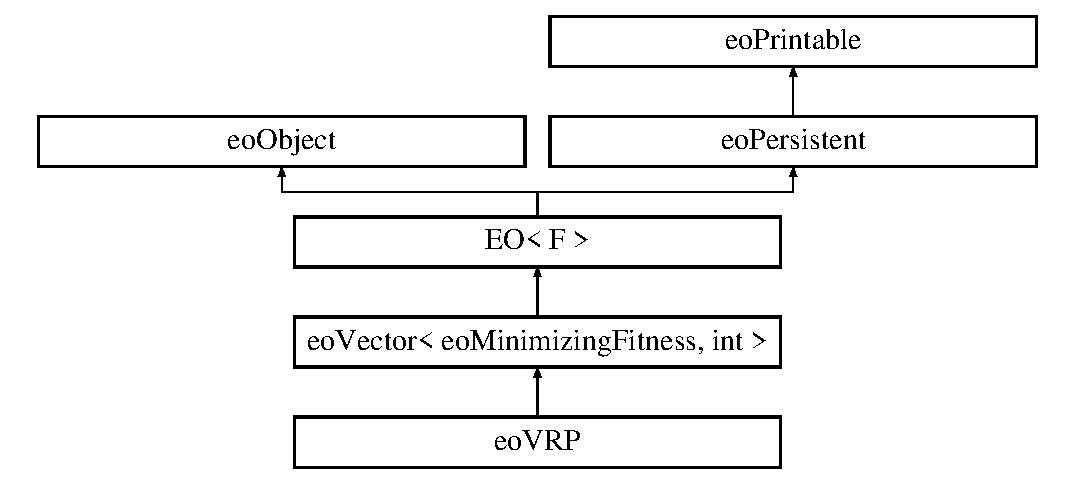
\includegraphics[height=5cm]{classeo_v_r_p}
\end{center}
\end{figure}
\subsection*{Public Member Functions}
\begin{CompactItemize}
\item 
\bf{eo\-VRP} ()\label{classeo_v_r_p_20e79a2ad5721ce7f2fe4a88f00692de}

\begin{CompactList}\small\item\em Default constructor: initializes variables to safe values. \item\end{CompactList}\item 
\bf{eo\-VRP} (const \bf{eo\-VRP} \&\_\-orig)
\begin{CompactList}\small\item\em Copy contructor: creates a new individual from a given one. \item\end{CompactList}\item 
virtual \bf{$\sim$eo\-VRP} ()\label{classeo_v_r_p_dedbd3437656d5dacafab6652219c8e2}

\begin{CompactList}\small\item\em Default destructor: nothing to do here. \item\end{CompactList}\item 
\bf{eo\-VRP} \& \bf{operator=} (const \bf{eo\-VRP} \&\_\-orig)
\begin{CompactList}\small\item\em Performs a copy from the invidual passed as argument. \item\end{CompactList}\item 
virtual std::string \bf{class\-Name} () const 
\begin{CompactList}\small\item\em Returns a string containing the name of the class. \item\end{CompactList}\item 
void \bf{print\-On} (std::ostream \&\_\-os) const 
\begin{CompactList}\small\item\em Prints the individual to a given stream. \item\end{CompactList}\item 
void \bf{print\-All\-On} (std::ostream \&\_\-os) const 
\begin{CompactList}\small\item\em Prints a detailed version of the individual (decoding information, unsatisfied contraints, etc. \item\end{CompactList}\item 
void \bf{read\-From} (std::istream \&\_\-is)
\begin{CompactList}\small\item\em Reads an individual from a given stream. \item\end{CompactList}\item 
const Routes \& \bf{routes} ()
\begin{CompactList}\small\item\em Returns a reference to the decoded individual. \item\end{CompactList}\item 
double \bf{length} ()
\begin{CompactList}\small\item\em Returns the total cost (length) of traveling all the routes. \item\end{CompactList}\item 
void \bf{print\-Routes} (std::ostream \&\_\-os) const 
\begin{CompactList}\small\item\em Aux. \item\end{CompactList}\item 
void \bf{print\-Route} (std::ostream \&\_\-os, unsigned \_\-p) const 
\begin{CompactList}\small\item\em Aux. \item\end{CompactList}\item 
bool \bf{clean} ()
\begin{CompactList}\small\item\em Cleans the individual (the vector of clients and also the decoding information). \item\end{CompactList}\item 
bool \bf{clean\-Routes} ()
\begin{CompactList}\small\item\em Invalidates the decoding information (usually after crossover or mutation). \item\end{CompactList}\item 
bool \bf{decoded} () const 
\begin{CompactList}\small\item\em Has this individual been decoded? \item\end{CompactList}\item 
bool \bf{encode} (Routes \&\_\-routes)
\begin{CompactList}\small\item\em Encodes an individual from a set of routes (usually used within crossover). \item\end{CompactList}\item 
double \bf{decode} ()
\begin{CompactList}\small\item\em Decodes an individual in a set of routes and calculates its cost (length) of traveling. \item\end{CompactList}\end{CompactItemize}
\subsection*{Private Attributes}
\begin{CompactItemize}
\item 
Routes \bf{m\-Routes}\label{classeo_v_r_p_ecbcda9f187d0d842c043544daa33558}

\begin{CompactList}\small\item\em A set of routes containing the decoding information of the individual. \item\end{CompactList}\item 
double \bf{m\-Length}\label{classeo_v_r_p_0e8c40e00bd835dd380d26d4a3abf544}

\begin{CompactList}\small\item\em Cached cost (length) of traveling the set of routes defined by the individual. \item\end{CompactList}\end{CompactItemize}


\subsection{Detailed Description}
Defines the getoype used to solve the VRP-TW problem. 



Definition at line 50 of file eo\-VRP.h.

\subsection{Constructor \& Destructor Documentation}
\index{eoVRP@{eo\-VRP}!eoVRP@{eoVRP}}
\index{eoVRP@{eoVRP}!eoVRP@{eo\-VRP}}
\subsubsection{\setlength{\rightskip}{0pt plus 5cm}eo\-VRP::eo\-VRP (const \bf{eo\-VRP} \& {\em \_\-orig})\hspace{0.3cm}{\tt  [inline]}}\label{classeo_v_r_p_1733318610dff5f47ac7d1272a4b4fb1}


Copy contructor: creates a new individual from a given one. 

\begin{Desc}
\item[Parameters:]
\begin{description}
\item[{\em \_\-orig}]The individual used to create the new one. \end{description}
\end{Desc}


Definition at line 68 of file eo\-VRP.h.

References operator=().

\subsection{Member Function Documentation}
\index{eoVRP@{eo\-VRP}!operator=@{operator=}}
\index{operator=@{operator=}!eoVRP@{eo\-VRP}}
\subsubsection{\setlength{\rightskip}{0pt plus 5cm}\bf{eo\-VRP}\& eo\-VRP::operator= (const \bf{eo\-VRP} \& {\em \_\-orig})\hspace{0.3cm}{\tt  [inline]}}\label{classeo_v_r_p_c0fcb2c17f849bfa61dd5d7ff072e0e4}


Performs a copy from the invidual passed as argument. 

\begin{Desc}
\item[Parameters:]
\begin{description}
\item[{\em \_\-orig}]The individual to copy from. \end{description}
\end{Desc}
\begin{Desc}
\item[Returns:]A reference to this. \end{Desc}


Definition at line 90 of file eo\-VRP.h.

References clean(), m\-Length, and m\-Routes.

Referenced by eo\-VRP().\index{eoVRP@{eo\-VRP}!className@{className}}
\index{className@{className}!eoVRP@{eo\-VRP}}
\subsubsection{\setlength{\rightskip}{0pt plus 5cm}virtual std::string eo\-VRP::class\-Name (void) const\hspace{0.3cm}{\tt  [inline, virtual]}}\label{classeo_v_r_p_8c7f524cf34787f9ec26ffcc420565c5}


Returns a string containing the name of the class. 

\begin{Desc}
\item[Returns:]The string containing the name of the class. \end{Desc}


Reimplemented from \bf{EO$<$ F $>$}.

Definition at line 117 of file eo\-VRP.h.\index{eoVRP@{eo\-VRP}!printOn@{printOn}}
\index{printOn@{printOn}!eoVRP@{eo\-VRP}}
\subsubsection{\setlength{\rightskip}{0pt plus 5cm}void eo\-VRP::print\-On (std::ostream \& {\em \_\-os}) const\hspace{0.3cm}{\tt  [inline, virtual]}}\label{classeo_v_r_p_dc4cb13768ef1a2c810d4d298b36707c}


Prints the individual to a given stream. 

\begin{Desc}
\item[Parameters:]
\begin{description}
\item[{\em \_\-os}]The stream to print to. \end{description}
\end{Desc}


Reimplemented from \bf{eo\-Vector$<$ eo\-Minimizing\-Fitness, int $>$}.

Definition at line 129 of file eo\-VRP.h.

References eo\-Vector$<$ Fit\-T, Gene\-Type $>$::print\-On().

Referenced by decode().\index{eoVRP@{eo\-VRP}!printAllOn@{printAllOn}}
\index{printAllOn@{printAllOn}!eoVRP@{eo\-VRP}}
\subsubsection{\setlength{\rightskip}{0pt plus 5cm}void eo\-VRP::print\-All\-On (std::ostream \& {\em \_\-os}) const\hspace{0.3cm}{\tt  [inline]}}\label{classeo_v_r_p_738f0aa43d8608cc68e41b1d3f8c944d}


Prints a detailed version of the individual (decoding information, unsatisfied contraints, etc. 

) to a given stream. \begin{Desc}
\item[Parameters:]
\begin{description}
\item[{\em \_\-os}]The stream to print to. \end{description}
\end{Desc}


Definition at line 146 of file eo\-VRP.h.

References decoded(), EO$<$ F $>$::fitness(), eo\-Vector$<$ Fit\-T, Gene\-Type $>$::print\-On(), and print\-Routes().\index{eoVRP@{eo\-VRP}!readFrom@{readFrom}}
\index{readFrom@{readFrom}!eoVRP@{eo\-VRP}}
\subsubsection{\setlength{\rightskip}{0pt plus 5cm}void eo\-VRP::read\-From (std::istream \& {\em \_\-is})\hspace{0.3cm}{\tt  [inline, virtual]}}\label{classeo_v_r_p_fdb87ffaf7ac95988e8896bb896183cc}


Reads an individual from a given stream. 

\begin{Desc}
\item[Parameters:]
\begin{description}
\item[{\em \_\-is}]The stream to read from. \end{description}
\end{Desc}


Reimplemented from \bf{eo\-Vector$<$ eo\-Minimizing\-Fitness, int $>$}.

Definition at line 177 of file eo\-VRP.h.

References eo\-Vector$<$ Fit\-T, Gene\-Type $>$::read\-From().\index{eoVRP@{eo\-VRP}!routes@{routes}}
\index{routes@{routes}!eoVRP@{eo\-VRP}}
\subsubsection{\setlength{\rightskip}{0pt plus 5cm}const Routes\& eo\-VRP::routes ()\hspace{0.3cm}{\tt  [inline]}}\label{classeo_v_r_p_0e000044813b4ebdd822e7e2f8540d8b}


Returns a reference to the decoded individual. 

\begin{Desc}
\item[Returns:]A reference to the decoded individual. \end{Desc}


Definition at line 190 of file eo\-VRP.h.

References m\-Routes.

Referenced by eo\-VRPGeneric\-Crossover::operator()().\index{eoVRP@{eo\-VRP}!length@{length}}
\index{length@{length}!eoVRP@{eo\-VRP}}
\subsubsection{\setlength{\rightskip}{0pt plus 5cm}double eo\-VRP::length ()\hspace{0.3cm}{\tt  [inline]}}\label{classeo_v_r_p_e4d189ca6349a875ae8d6fd9c7fe2491}


Returns the total cost (length) of traveling all the routes. 

\begin{Desc}
\item[Returns:]The total cost (length) of traveling all the routes. \end{Desc}


Definition at line 205 of file eo\-VRP.h.

References m\-Length.

Referenced by eo\-VRPEval\-Func::operator()().\index{eoVRP@{eo\-VRP}!printRoutes@{printRoutes}}
\index{printRoutes@{printRoutes}!eoVRP@{eo\-VRP}}
\subsubsection{\setlength{\rightskip}{0pt plus 5cm}void eo\-VRP::print\-Routes (std::ostream \& {\em \_\-os}) const\hspace{0.3cm}{\tt  [inline]}}\label{classeo_v_r_p_2a4c249cc6b15819c48c9210db385dc7}


Aux. 

method to print a structure of routes. \begin{Desc}
\item[Parameters:]
\begin{description}
\item[{\em \_\-os}]The stream to print to. \end{description}
\end{Desc}


Definition at line 217 of file eo\-VRP.h.

References m\-Routes, and print\-Route().

Referenced by print\-All\-On().\index{eoVRP@{eo\-VRP}!printRoute@{printRoute}}
\index{printRoute@{printRoute}!eoVRP@{eo\-VRP}}
\subsubsection{\setlength{\rightskip}{0pt plus 5cm}void eo\-VRP::print\-Route (std::ostream \& {\em \_\-os}, unsigned {\em \_\-p}) const\hspace{0.3cm}{\tt  [inline]}}\label{classeo_v_r_p_ec256ed5b3b15b6d220494015e2aba93}


Aux. 

method to print only one route. \begin{Desc}
\item[Parameters:]
\begin{description}
\item[{\em \_\-os}]The stream to print to. \item[{\em \_\-p}]The route to print. \end{description}
\end{Desc}


Definition at line 244 of file eo\-VRP.h.

References m\-Routes.

Referenced by print\-Routes().\index{eoVRP@{eo\-VRP}!clean@{clean}}
\index{clean@{clean}!eoVRP@{eo\-VRP}}
\subsubsection{\setlength{\rightskip}{0pt plus 5cm}bool eo\-VRP::clean ()\hspace{0.3cm}{\tt  [inline]}}\label{classeo_v_r_p_1c53a7a42174c7d40db92da644b25fec}


Cleans the individual (the vector of clients and also the decoding information). 

\begin{Desc}
\item[Returns:]True if the operation finishes correctly. False otherwise. \end{Desc}


Definition at line 267 of file eo\-VRP.h.

References m\-Length, and m\-Routes.

Referenced by encode(), eo\-VRPEdge\-Crossover::operator()(), and operator=().\index{eoVRP@{eo\-VRP}!cleanRoutes@{cleanRoutes}}
\index{cleanRoutes@{cleanRoutes}!eoVRP@{eo\-VRP}}
\subsubsection{\setlength{\rightskip}{0pt plus 5cm}bool eo\-VRP::clean\-Routes ()\hspace{0.3cm}{\tt  [inline]}}\label{classeo_v_r_p_66fb699c1d34cac859406ad450be406a}


Invalidates the decoding information (usually after crossover or mutation). 

\begin{Desc}
\item[Returns:]True if the operation finishes correctly. False otherwise. \end{Desc}


Definition at line 283 of file eo\-VRP.h.

References m\-Length, and m\-Routes.

Referenced by decode(), eo\-VRPOne\-Point\-Crossover::operator()(), and eo\-VRPMutation::operator()().\index{eoVRP@{eo\-VRP}!decoded@{decoded}}
\index{decoded@{decoded}!eoVRP@{eo\-VRP}}
\subsubsection{\setlength{\rightskip}{0pt plus 5cm}bool eo\-VRP::decoded () const\hspace{0.3cm}{\tt  [inline]}}\label{classeo_v_r_p_e188fadc91b4ee256e144ac86ee80a40}


Has this individual been decoded? 

\begin{Desc}
\item[Returns:]True if has decoding information. False otherwise. \end{Desc}


Definition at line 298 of file eo\-VRP.h.

References m\-Routes.

Referenced by eo\-VRPEval\-Func::operator()(), and print\-All\-On().\index{eoVRP@{eo\-VRP}!encode@{encode}}
\index{encode@{encode}!eoVRP@{eo\-VRP}}
\subsubsection{\setlength{\rightskip}{0pt plus 5cm}bool eo\-VRP::encode (Routes \& {\em \_\-routes})\hspace{0.3cm}{\tt  [inline]}}\label{classeo_v_r_p_b56c820bff344b4cd7338628a6f8f083}


Encodes an individual from a set of routes (usually used within crossover). 

\begin{Desc}
\item[Returns:]True if the operation finishes correctly. False otherwise. \end{Desc}


Definition at line 313 of file eo\-VRP.h.

References clean().

Referenced by eo\-VRPGeneric\-Crossover::operator()().\index{eoVRP@{eo\-VRP}!decode@{decode}}
\index{decode@{decode}!eoVRP@{eo\-VRP}}
\subsubsection{\setlength{\rightskip}{0pt plus 5cm}double eo\-VRP::decode ()\hspace{0.3cm}{\tt  [inline]}}\label{classeo_v_r_p_fdfd2633515baa85c3fdaf39be6dea5c}


Decodes an individual in a set of routes and calculates its cost (length) of traveling. 

\begin{Desc}
\item[Returns:]The cost (length) of traveling the set of routes. \end{Desc}


Definition at line 334 of file eo\-VRP.h.

References clean\-Routes(), eo\-VRPUtils::clients, eo\-VRPUtils::distance(), eo\-VRPUtils::get\-Time\-Window(), m\-Length, m\-Routes, and print\-On().

Referenced by eo\-VRPEval\-Func::operator()().

The documentation for this class was generated from the following file:\begin{CompactItemize}
\item 
eo\-VRP.h\end{CompactItemize}

\section{eo\-VRPEdge\-Crossover Class Reference}
\label{classeo_v_r_p_edge_crossover}\index{eoVRPEdgeCrossover@{eoVRPEdgeCrossover}}
Implementation of the classic Edge Crossover from the TSP.  


{\tt \#include $<$eo\-VRPQuad\-Crossover.h$>$}

Inheritance diagram for eo\-VRPEdge\-Crossover::\begin{figure}[H]
\begin{center}
\leavevmode
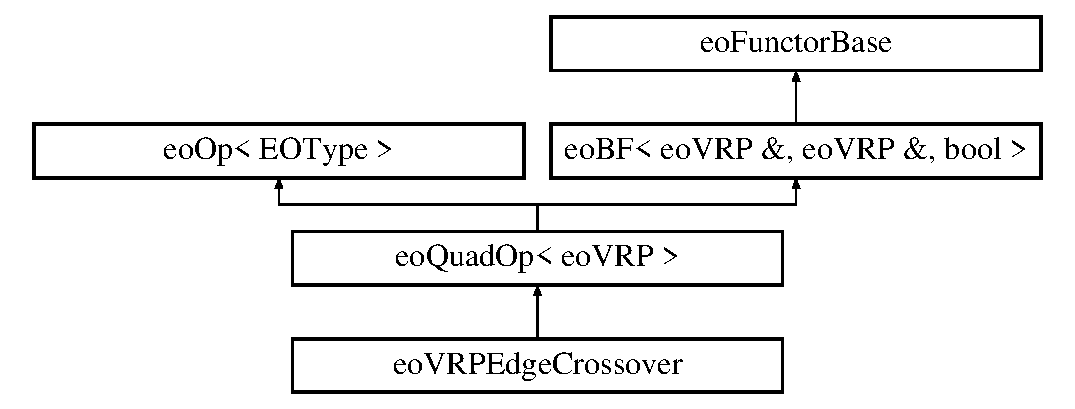
\includegraphics[height=4cm]{classeo_v_r_p_edge_crossover}
\end{center}
\end{figure}
\subsection*{Public Member Functions}
\begin{CompactItemize}
\item 
\bf{eo\-VRPEdge\-Crossover} ()\label{classeo_v_r_p_edge_crossover_1cec73fc43837a61b6c97812dd57891b}

\begin{CompactList}\small\item\em Deafult constructor. \item\end{CompactList}\item 
std::string \bf{class\-Name} () const 
\begin{CompactList}\small\item\em Returns a string containing the name of the class. \item\end{CompactList}\item 
bool \bf{operator()} (\bf{eo\-VRP} \&\_\-genotype1, \bf{eo\-VRP} \&\_\-genotype2)
\begin{CompactList}\small\item\em Both parameters are the parents and the (future) children of the crossover. \item\end{CompactList}\end{CompactItemize}
\subsection*{Private Member Functions}
\begin{CompactItemize}
\item 
bool \bf{Edge\-Crossover} (\bf{eo\-VRP} \&\_\-genotype1, \bf{eo\-VRP} \&\_\-genotype2, \bf{eo\-VRP} \&\_\-child)
\begin{CompactList}\small\item\em Actually performs the edge crossover. \item\end{CompactList}\item 
void \bf{remove\_\-entry} (unsigned \_\-vertex, std::vector$<$ std::set$<$ unsigned $>$ $>$ \&\_\-map)
\begin{CompactList}\small\item\em Removes a vertex from all his neighbours. \item\end{CompactList}\item 
void \bf{add\_\-vertex} (unsigned \_\-vertex, std::vector$<$ bool $>$ \&\_\-visited, std::vector$<$ std::set$<$ unsigned $>$ $>$ \&\_\-map, \bf{eo\-VRP} \&\_\-child)
\begin{CompactList}\small\item\em Adds a vertex to a child and erases it from the list of available vertices. \item\end{CompactList}\end{CompactItemize}


\subsection{Detailed Description}
Implementation of the classic Edge Crossover from the TSP. 



Definition at line 240 of file eo\-VRPQuad\-Crossover.h.

\subsection{Member Function Documentation}
\index{eoVRPEdgeCrossover@{eo\-VRPEdge\-Crossover}!className@{className}}
\index{className@{className}!eoVRPEdgeCrossover@{eo\-VRPEdge\-Crossover}}
\subsubsection{\setlength{\rightskip}{0pt plus 5cm}std::string eo\-VRPEdge\-Crossover::class\-Name (void) const\hspace{0.3cm}{\tt  [inline, virtual]}}\label{classeo_v_r_p_edge_crossover_8b2a199b70442852f93b2a34a42cf1e4}


Returns a string containing the name of the class. 

Used to display statistics. \begin{Desc}
\item[Returns:]The string containing the name of the class. \end{Desc}


Reimplemented from \bf{eo\-Quad\-Op$<$ eo\-VRP $>$}.

Definition at line 258 of file eo\-VRPQuad\-Crossover.h.\index{eoVRPEdgeCrossover@{eo\-VRPEdge\-Crossover}!operator()@{operator()}}
\index{operator()@{operator()}!eoVRPEdgeCrossover@{eo\-VRPEdge\-Crossover}}
\subsubsection{\setlength{\rightskip}{0pt plus 5cm}bool eo\-VRPEdge\-Crossover::operator() (\bf{eo\-VRP} \& {\em \_\-genotype1}, \bf{eo\-VRP} \& {\em \_\-genotype2})\hspace{0.3cm}{\tt  [inline, virtual]}}\label{classeo_v_r_p_edge_crossover_518856969ec708a73e728d36ddf01d1b}


Both parameters are the parents and the (future) children of the crossover. 

\begin{Desc}
\item[Parameters:]
\begin{description}
\item[{\em \_\-genotype1}]The first parent. \item[{\em \_\-genotype2}]The second parent. \end{description}
\end{Desc}
\begin{Desc}
\item[Returns:]True if any of the parents was modified. False otherwise. \end{Desc}


Implements \bf{eo\-BF$<$ eo\-VRP \&, eo\-VRP \&, bool $>$}.

Definition at line 272 of file eo\-VRPQuad\-Crossover.h.

References eo\-VRP::clean(), and Edge\-Crossover().\index{eoVRPEdgeCrossover@{eo\-VRPEdge\-Crossover}!EdgeCrossover@{EdgeCrossover}}
\index{EdgeCrossover@{EdgeCrossover}!eoVRPEdgeCrossover@{eo\-VRPEdge\-Crossover}}
\subsubsection{\setlength{\rightskip}{0pt plus 5cm}bool eo\-VRPEdge\-Crossover::Edge\-Crossover (\bf{eo\-VRP} \& {\em \_\-genotype1}, \bf{eo\-VRP} \& {\em \_\-genotype2}, \bf{eo\-VRP} \& {\em \_\-child})\hspace{0.3cm}{\tt  [inline, private]}}\label{classeo_v_r_p_edge_crossover_389bd29cab9e12915d0d5c4af80343d7}


Actually performs the edge crossover. 

\begin{Desc}
\item[Parameters:]
\begin{description}
\item[{\em \_\-genotype1}]First parent. \item[{\em \_\-genotype2}]Second parent. \item[{\em \_\-child}]Child. \end{description}
\end{Desc}
\begin{Desc}
\item[Returns:]True if the second parent was modified. False otherwise. \end{Desc}


Definition at line 301 of file eo\-VRPQuad\-Crossover.h.

References add\_\-vertex(), and eo\-Rng::random().

Referenced by operator()().\index{eoVRPEdgeCrossover@{eo\-VRPEdge\-Crossover}!remove_entry@{remove\_\-entry}}
\index{remove_entry@{remove\_\-entry}!eoVRPEdgeCrossover@{eo\-VRPEdge\-Crossover}}
\subsubsection{\setlength{\rightskip}{0pt plus 5cm}void eo\-VRPEdge\-Crossover::remove\_\-entry (unsigned {\em \_\-vertex}, std::vector$<$ std::set$<$ unsigned $>$ $>$ \& {\em \_\-map})\hspace{0.3cm}{\tt  [inline, private]}}\label{classeo_v_r_p_edge_crossover_df9886f80565a966c78fb5a08e12631f}


Removes a vertex from all his neighbours. 

\begin{Desc}
\item[Parameters:]
\begin{description}
\item[{\em \_\-vertex}]The vertex being erased. \item[{\em \_\-map}]The structure containing the neighbourhood relationship. \end{description}
\end{Desc}


Definition at line 380 of file eo\-VRPQuad\-Crossover.h.

Referenced by add\_\-vertex().\index{eoVRPEdgeCrossover@{eo\-VRPEdge\-Crossover}!add_vertex@{add\_\-vertex}}
\index{add_vertex@{add\_\-vertex}!eoVRPEdgeCrossover@{eo\-VRPEdge\-Crossover}}
\subsubsection{\setlength{\rightskip}{0pt plus 5cm}void eo\-VRPEdge\-Crossover::add\_\-vertex (unsigned {\em \_\-vertex}, std::vector$<$ bool $>$ \& {\em \_\-visited}, std::vector$<$ std::set$<$ unsigned $>$ $>$ \& {\em \_\-map}, \bf{eo\-VRP} \& {\em \_\-child})\hspace{0.3cm}{\tt  [inline, private]}}\label{classeo_v_r_p_edge_crossover_7917ea1dec6221f71127c6fae9515e68}


Adds a vertex to a child and erases it from the list of available vertices. 

\begin{Desc}
\item[Parameters:]
\begin{description}
\item[{\em \_\-vertex}]The vertex being added to the child. \item[{\em \_\-visited}]The vector of visited vertices. \item[{\em \_\-map}]The structure containing the neighbourhood relationship. \item[{\em \_\-child}]The child where we add the vertex. \end{description}
\end{Desc}


Definition at line 398 of file eo\-VRPQuad\-Crossover.h.

References remove\_\-entry().

Referenced by Edge\-Crossover().

The documentation for this class was generated from the following file:\begin{CompactItemize}
\item 
eo\-VRPQuad\-Crossover.h\end{CompactItemize}

\section{eo\-VRPEval\-Func Class Reference}
\label{classeo_v_r_p_eval_func}\index{eoVRPEvalFunc@{eoVRPEvalFunc}}
Evaluates an individual of type \doxyref{eo\-VRP}{p.}{classeo_v_r_p}.  


{\tt \#include $<$eo\-VRPEval\-Func.h$>$}

Inheritance diagram for eo\-VRPEval\-Func::\begin{figure}[H]
\begin{center}
\leavevmode
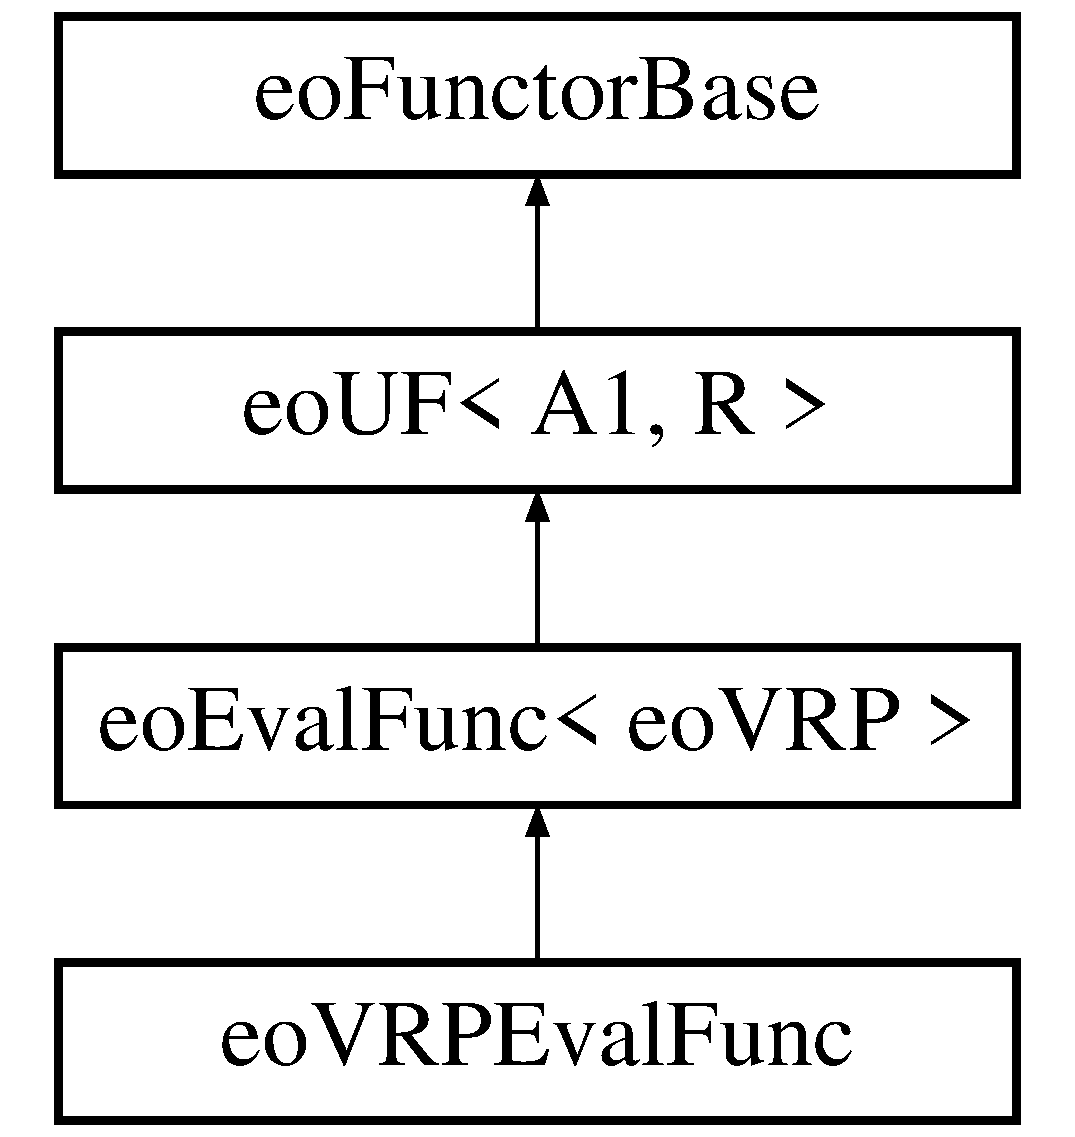
\includegraphics[height=4cm]{classeo_v_r_p_eval_func}
\end{center}
\end{figure}
\subsection*{Public Member Functions}
\begin{CompactItemize}
\item 
\bf{eo\-VRPEval\-Func} ()\label{classeo_v_r_p_eval_func_9746622fd0ae11ae58261b0711b7918c}

\begin{CompactList}\small\item\em Constructor: nothing to do here. \item\end{CompactList}\item 
void \bf{operator()} (\bf{eo\-VRP} \&\_\-eo)
\begin{CompactList}\small\item\em Computes the (penalized) fitness. \item\end{CompactList}\end{CompactItemize}


\subsection{Detailed Description}
Evaluates an individual of type \doxyref{eo\-VRP}{p.}{classeo_v_r_p}. 



Definition at line 54 of file eo\-VRPEval\-Func.h.

\subsection{Member Function Documentation}
\index{eoVRPEvalFunc@{eo\-VRPEval\-Func}!operator()@{operator()}}
\index{operator()@{operator()}!eoVRPEvalFunc@{eo\-VRPEval\-Func}}
\subsubsection{\setlength{\rightskip}{0pt plus 5cm}void eo\-VRPEval\-Func::operator() (\bf{eo\-VRP} \& {\em \_\-eo})\hspace{0.3cm}{\tt  [inline]}}\label{classeo_v_r_p_eval_func_840c1a7d38dbdeb40e283df3be42aa48}


Computes the (penalized) fitness. 

\begin{Desc}
\item[Parameters:]
\begin{description}
\item[{\em \_\-eo}]The individual to be evaluated. \end{description}
\end{Desc}


Definition at line 72 of file eo\-VRPEval\-Func.h.

References eo\-VRP::decode(), eo\-VRP::decoded(), EO$<$ F $>$::fitness(), EO$<$ F $>$::invalid(), and eo\-VRP::length().

The documentation for this class was generated from the following file:\begin{CompactItemize}
\item 
eo\-VRPEval\-Func.h\end{CompactItemize}

\section{eo\-VRPGeneric\-Crossover Class Reference}
\label{classeo_v_r_p_generic_crossover}\index{eoVRPGenericCrossover@{eoVRPGenericCrossover}}
Implementation of the generic crossover for the VRP-TW by Tavares et al.  


{\tt \#include $<$eo\-VRPQuad\-Crossover.h$>$}

Inheritance diagram for eo\-VRPGeneric\-Crossover::\begin{figure}[H]
\begin{center}
\leavevmode
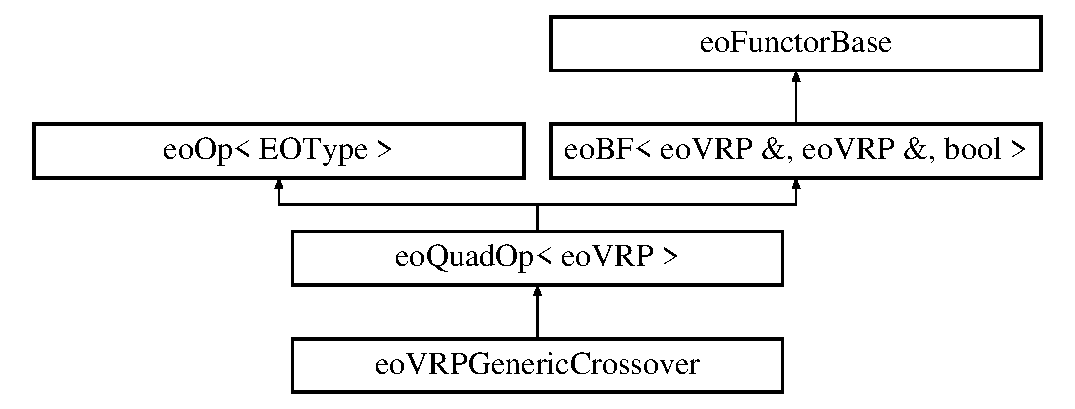
\includegraphics[height=4cm]{classeo_v_r_p_generic_crossover}
\end{center}
\end{figure}
\subsection*{Public Member Functions}
\begin{CompactItemize}
\item 
\bf{eo\-VRPGeneric\-Crossover} ()\label{classeo_v_r_p_generic_crossover_63e5fb734c46be62a12f6799e34cebe4}

\begin{CompactList}\small\item\em Deafult constructor. \item\end{CompactList}\item 
std::string \bf{class\-Name} () const 
\begin{CompactList}\small\item\em Returns a string containing the name of the class. \item\end{CompactList}\item 
bool \bf{operator()} (\bf{eo\-VRP} \&\_\-genotype1, \bf{eo\-VRP} \&\_\-genotype2)
\begin{CompactList}\small\item\em Both parameters are the parents and the (future) children of the crossover. \item\end{CompactList}\end{CompactItemize}
\subsection*{Private Member Functions}
\begin{CompactItemize}
\item 
bool \bf{Generic\-Crossover} (const Routes \&\_\-donor, Routes \&\_\-receiver) const 
\begin{CompactList}\small\item\em Actually performs the generic crossover. \item\end{CompactList}\end{CompactItemize}


\subsection{Detailed Description}
Implementation of the generic crossover for the VRP-TW by Tavares et al. 



Definition at line 53 of file eo\-VRPQuad\-Crossover.h.

\subsection{Member Function Documentation}
\index{eoVRPGenericCrossover@{eo\-VRPGeneric\-Crossover}!className@{className}}
\index{className@{className}!eoVRPGenericCrossover@{eo\-VRPGeneric\-Crossover}}
\subsubsection{\setlength{\rightskip}{0pt plus 5cm}std::string eo\-VRPGeneric\-Crossover::class\-Name (void) const\hspace{0.3cm}{\tt  [inline, virtual]}}\label{classeo_v_r_p_generic_crossover_7740db73b7151dab52df9d50f5366429}


Returns a string containing the name of the class. 

Used to display statistics. \begin{Desc}
\item[Returns:]The string containing the name of the class. \end{Desc}


Reimplemented from \bf{eo\-Quad\-Op$<$ eo\-VRP $>$}.

Definition at line 71 of file eo\-VRPQuad\-Crossover.h.\index{eoVRPGenericCrossover@{eo\-VRPGeneric\-Crossover}!operator()@{operator()}}
\index{operator()@{operator()}!eoVRPGenericCrossover@{eo\-VRPGeneric\-Crossover}}
\subsubsection{\setlength{\rightskip}{0pt plus 5cm}bool eo\-VRPGeneric\-Crossover::operator() (\bf{eo\-VRP} \& {\em \_\-genotype1}, \bf{eo\-VRP} \& {\em \_\-genotype2})\hspace{0.3cm}{\tt  [inline, virtual]}}\label{classeo_v_r_p_generic_crossover_d7d3b19562b071bd50dd4d831e447d0c}


Both parameters are the parents and the (future) children of the crossover. 

\begin{Desc}
\item[Parameters:]
\begin{description}
\item[{\em \_\-genotype1}]The first parent. \item[{\em \_\-genotype2}]The second parent. \end{description}
\end{Desc}
\begin{Desc}
\item[Returns:]True if any of the parents was modified. False otherwise. \end{Desc}


Implements \bf{eo\-BF$<$ eo\-VRP \&, eo\-VRP \&, bool $>$}.

Definition at line 85 of file eo\-VRPQuad\-Crossover.h.

References eo\-VRP::encode(), Generic\-Crossover(), and eo\-VRP::routes().\index{eoVRPGenericCrossover@{eo\-VRPGeneric\-Crossover}!GenericCrossover@{GenericCrossover}}
\index{GenericCrossover@{GenericCrossover}!eoVRPGenericCrossover@{eo\-VRPGeneric\-Crossover}}
\subsubsection{\setlength{\rightskip}{0pt plus 5cm}bool eo\-VRPGeneric\-Crossover::Generic\-Crossover (const Routes \& {\em \_\-donor}, Routes \& {\em \_\-receiver}) const\hspace{0.3cm}{\tt  [inline, private]}}\label{classeo_v_r_p_generic_crossover_543ba6869b93a3f9f709045b7e24d74a}


Actually performs the generic crossover. 

\begin{Desc}
\item[Parameters:]
\begin{description}
\item[{\em \_\-donor}]Set of routes from the first parent. \item[{\em \_\-receiver}]Set of routes from the second parent \end{description}
\end{Desc}
\begin{Desc}
\item[Returns:]True if the second parent was modified. False otherwise. \end{Desc}


Definition at line 110 of file eo\-VRPQuad\-Crossover.h.

References eo\-Rng::random().

Referenced by operator()().

The documentation for this class was generated from the following file:\begin{CompactItemize}
\item 
eo\-VRPQuad\-Crossover.h\end{CompactItemize}

\section{eo\-VRPInit Class Reference}
\label{classeo_v_r_p_init}\index{eoVRPInit@{eoVRPInit}}
Class defining the initializer functor.  


{\tt \#include $<$eo\-VRPInit.h$>$}

Inheritance diagram for eo\-VRPInit::\begin{figure}[H]
\begin{center}
\leavevmode
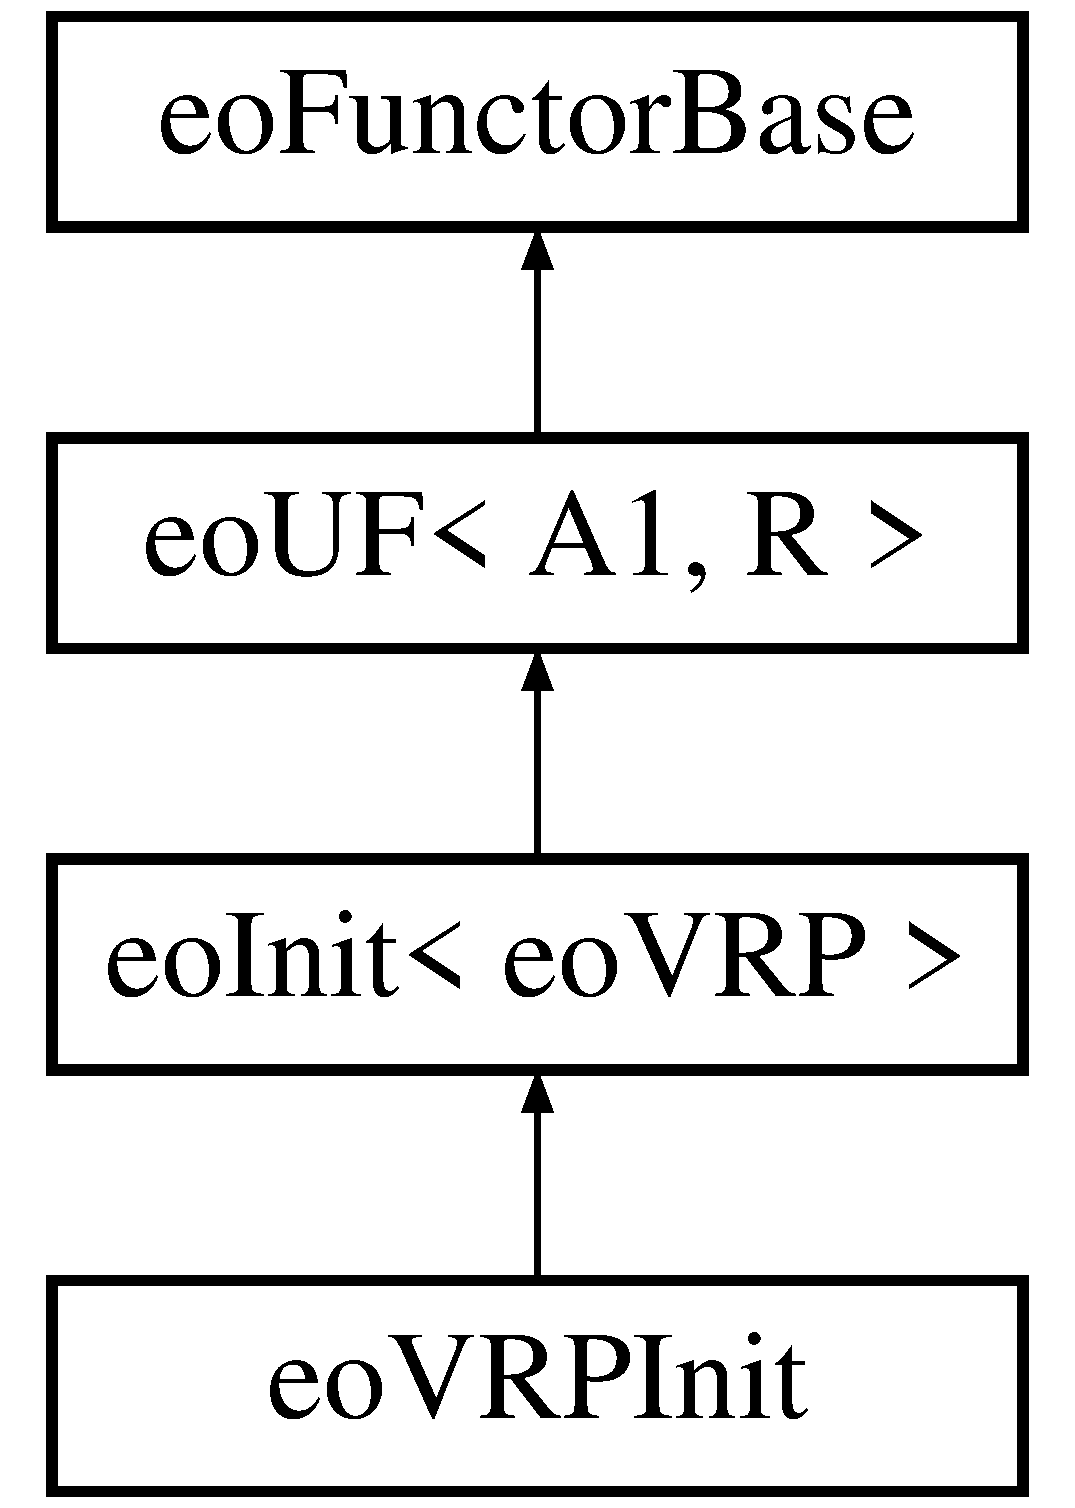
\includegraphics[height=4cm]{classeo_v_r_p_init}
\end{center}
\end{figure}
\subsection*{Public Member Functions}
\begin{CompactItemize}
\item 
\bf{eo\-VRPInit} ()\label{classeo_v_r_p_init_a620d4fa1b930b1fd8b491f1ef5c72fd}

\begin{CompactList}\small\item\em Default constructor: nothing to do here. \item\end{CompactList}\item 
void \bf{operator()} (\bf{eo\-VRP} \&\_\-gen)
\begin{CompactList}\small\item\em Functor member. \item\end{CompactList}\end{CompactItemize}
\subsection*{Private Member Functions}
\begin{CompactItemize}
\item 
void \bf{Heuristic\-Initialization} (\bf{eo\-VRP} \&\_\-gen)
\begin{CompactList}\small\item\em Heuristic initializer. \item\end{CompactList}\item 
bool \bf{create\-New\-Route} (std::vector$<$ int $>$ \&\_\-unvisited, int \&\_\-unvisited\-Idx, bool \_\-seed\-Checking\-Override, Route \&\_\-route)
\begin{CompactList}\small\item\em Creates a new route. \item\end{CompactList}\item 
bool \bf{select\-Best\-Insertion} (std::vector$<$ int $>$ \&\_\-unvisited, unsigned \_\-unvisited\-Idx, Route \&\_\-route, unsigned \&\_\-next\-Client, Route::iterator \&\_\-it)
\begin{CompactList}\small\item\em Selects the best client and the best position for its insertion in a given route. \item\end{CompactList}\item 
bool \bf{evaluate\-Insertion} (Route \&\_\-route, unsigned \_\-new\-Client, int \_\-after\-Client, double \&\_\-cost)
\begin{CompactList}\small\item\em Evaluates the feasibility and the cost of inserting a new client in a given subroute. \item\end{CompactList}\item 
unsigned \bf{select\-Farthest\-Client\-As\-Seed} (const std::vector$<$ int $>$ \&\_\-unvisited, int \_\-unvisited\-Idx)
\begin{CompactList}\small\item\em Selects the farthest client as seed for a new route. \item\end{CompactList}\item 
unsigned \bf{select\-Cheapest\-Client} (const std::vector$<$ int $>$ \&\_\-unvisited, int \_\-unvisited\-Idx, bool \_\-seed\-Checking\-Override)
\begin{CompactList}\small\item\em Selects the cheapest client as seed for a new route. \item\end{CompactList}\item 
unsigned \bf{select\-Best\-Client\-As\-Seed} (const std::vector$<$ int $>$ \&\_\-unvisited, int \_\-unvisited\-Idx, bool \_\-seed\-Checking\-Override)
\begin{CompactList}\small\item\em Selects the best (the \char`\"{}hardest\char`\"{} one) client as seed for a new route. \item\end{CompactList}\item 
void \bf{Random\-Initialization\-No\-Check} (\bf{eo\-VRP} \&\_\-gen)
\begin{CompactList}\small\item\em Random initializer. \item\end{CompactList}\end{CompactItemize}
\subsection*{Private Attributes}
\begin{CompactItemize}
\item 
unsigned \bf{m\-Seeds\-Used\-Count}\label{classeo_v_r_p_init_b74e164ca817fe5615e9519ec671a356}

\begin{CompactList}\small\item\em Number of clients already used as seeds. \item\end{CompactList}\item 
std::vector$<$ bool $>$ \bf{m\-Seeds\-Used}\label{classeo_v_r_p_init_5e940cc7eec88f268e8eb72313212947}

\begin{CompactList}\small\item\em Vector storing if a client has been used as a seed or not. \item\end{CompactList}\end{CompactItemize}


\subsection{Detailed Description}
Class defining the initializer functor. 

This class initializes an individual of the VRP problem using an heuristic initializer. 



Definition at line 65 of file eo\-VRPInit.h.

\subsection{Member Function Documentation}
\index{eoVRPInit@{eo\-VRPInit}!operator()@{operator()}}
\index{operator()@{operator()}!eoVRPInit@{eo\-VRPInit}}
\subsubsection{\setlength{\rightskip}{0pt plus 5cm}void eo\-VRPInit::operator() (\bf{eo\-VRP} \& {\em \_\-gen})\hspace{0.3cm}{\tt  [inline]}}\label{classeo_v_r_p_init_8bc4f6fb201b09dd882d721d2cfef8ce}


Functor member. 

Initializes a genotype using an heuristic initializer. \begin{Desc}
\item[Parameters:]
\begin{description}
\item[{\em \_\-gen}]Generally a genotype that has been default-constructed. Whatever it contains will be lost. \end{description}
\end{Desc}


Definition at line 99 of file eo\-VRPInit.h.

References Heuristic\-Initialization().\index{eoVRPInit@{eo\-VRPInit}!HeuristicInitialization@{HeuristicInitialization}}
\index{HeuristicInitialization@{HeuristicInitialization}!eoVRPInit@{eo\-VRPInit}}
\subsubsection{\setlength{\rightskip}{0pt plus 5cm}void eo\-VRPInit::Heuristic\-Initialization (\bf{eo\-VRP} \& {\em \_\-gen})\hspace{0.3cm}{\tt  [inline, private]}}\label{classeo_v_r_p_init_af5946da88fb14494cb23dc21d167866}


Heuristic initializer. 

This initializer constructs and individual from routes. Each route is built in a constructive way. The first client of each route is selected trying to maximize a function depending on its time window and how far it is from the depot. We always try to select the hardest clients as seeds. Used seeds are stored so that different seeds are selected for different individuals and thus guarantee the diversity of the initial population. \begin{Desc}
\item[Parameters:]
\begin{description}
\item[{\em \_\-gen}]The individual to be initialized. \end{description}
\end{Desc}


Definition at line 123 of file eo\-VRPInit.h.

References eo\-VRPUtils::clients, create\-New\-Route(), and EO$<$ F $>$::invalidate().

Referenced by operator()().\index{eoVRPInit@{eo\-VRPInit}!createNewRoute@{createNewRoute}}
\index{createNewRoute@{createNewRoute}!eoVRPInit@{eo\-VRPInit}}
\subsubsection{\setlength{\rightskip}{0pt plus 5cm}bool eo\-VRPInit::create\-New\-Route (std::vector$<$ int $>$ \& {\em \_\-unvisited}, int \& {\em \_\-unvisited\-Idx}, bool {\em \_\-seed\-Checking\-Override}, Route \& {\em \_\-route})\hspace{0.3cm}{\tt  [inline, private]}}\label{classeo_v_r_p_init_ff7c0bf38bdd70d6f9d561479ec4f48a}


Creates a new route. 

Creates a new route selecting the best (hardest) client as seed and then adding the cheapest clients until one of the constraints (time window or vehicle's capacity) is broken. \begin{Desc}
\item[Parameters:]
\begin{description}
\item[{\em \_\-unvisited}]Vector of unvisited and thus available clients for constructing the new route. \item[{\em \_\-unvisited\-Idx}]Position of the last univisted client in \_\-unvisited vector. \item[{\em \_\-seed\-Checking\-Override}]If true, it overrides the seed checking mecanism. It must be always false for the first route and then true for the following ones. This way we will preserve diversity in our initial population as every individual will be initialized from a different initial route. \item[{\em \_\-route}]The brand new route we have constructed. \end{description}
\end{Desc}
\begin{Desc}
\item[Returns:]True if everything went ok. \end{Desc}


Definition at line 176 of file eo\-VRPInit.h.

References m\-Seeds\-Used, m\-Seeds\-Used\-Count, select\-Best\-Client\-As\-Seed(), and select\-Best\-Insertion().

Referenced by Heuristic\-Initialization().\index{eoVRPInit@{eo\-VRPInit}!selectBestInsertion@{selectBestInsertion}}
\index{selectBestInsertion@{selectBestInsertion}!eoVRPInit@{eo\-VRPInit}}
\subsubsection{\setlength{\rightskip}{0pt plus 5cm}bool eo\-VRPInit::select\-Best\-Insertion (std::vector$<$ int $>$ \& {\em \_\-unvisited}, unsigned {\em \_\-unvisited\-Idx}, Route \& {\em \_\-route}, unsigned \& {\em \_\-next\-Client}, Route::iterator \& {\em \_\-it})\hspace{0.3cm}{\tt  [inline, private]}}\label{classeo_v_r_p_init_7f07be1f3a027dc56af84bb46828ddda}


Selects the best client and the best position for its insertion in a given route. 

Given a subroute, this method tries to find the best client and the best position for it among all the univisited clients. \begin{Desc}
\item[Parameters:]
\begin{description}
\item[{\em \_\-unvisited}]Vector of unvisited and thus available clients for constructing the new route. \item[{\em \_\-unvisited\-Idx}]Position of the last univisted client in \_\-unvisited vector. \item[{\em \_\-route}]The route where we are trying to insert a new client. \item[{\em \_\-next\-Client}]A return value. The selected client to be inserted. \item[{\em \_\-it}]A return value. The position for selected client to be inserted. \end{description}
\end{Desc}
\begin{Desc}
\item[Returns:]True if a new insertion is possible. False otherwise. \end{Desc}


Definition at line 249 of file eo\-VRPInit.h.

References evaluate\-Insertion().

Referenced by create\-New\-Route().\index{eoVRPInit@{eo\-VRPInit}!evaluateInsertion@{evaluateInsertion}}
\index{evaluateInsertion@{evaluateInsertion}!eoVRPInit@{eo\-VRPInit}}
\subsubsection{\setlength{\rightskip}{0pt plus 5cm}bool eo\-VRPInit::evaluate\-Insertion (Route \& {\em \_\-route}, unsigned {\em \_\-new\-Client}, int {\em \_\-after\-Client}, double \& {\em \_\-cost})\hspace{0.3cm}{\tt  [inline, private]}}\label{classeo_v_r_p_init_82f2bb762d8f5da85febd266fb75a29b}


Evaluates the feasibility and the cost of inserting a new client in a given subroute. 

Given a subroute, this method tries evaluates if it is possible to insert a client in a position. It will return the cost of the resulting route if this insertion is possible. \begin{Desc}
\item[Parameters:]
\begin{description}
\item[{\em \_\-route}]The route where we are trying to insert a new client. \item[{\em \_\-new\-Client}]The client we are trying to insert. \item[{\em \_\-after\-Client}]The position of insertion. \item[{\em \_\-cost}]A return value. The cost of inserting the given client at the given position. \end{description}
\end{Desc}
\begin{Desc}
\item[Returns:]True if the new insertion is possible. False otherwise. \end{Desc}


Definition at line 308 of file eo\-VRPInit.h.

References eo\-VRPUtils::clients, eo\-VRPUtils::distance(), and eo\-VRPUtils::get\-Time\-Window().

Referenced by select\-Best\-Insertion().\index{eoVRPInit@{eo\-VRPInit}!selectFarthestClientAsSeed@{selectFarthestClientAsSeed}}
\index{selectFarthestClientAsSeed@{selectFarthestClientAsSeed}!eoVRPInit@{eo\-VRPInit}}
\subsubsection{\setlength{\rightskip}{0pt plus 5cm}unsigned eo\-VRPInit::select\-Farthest\-Client\-As\-Seed (const std::vector$<$ int $>$ \& {\em \_\-unvisited}, int {\em \_\-unvisited\-Idx})\hspace{0.3cm}{\tt  [inline, private]}}\label{classeo_v_r_p_init_a24867d25a6c9911e9b5c9eb1b4b650d}


Selects the farthest client as seed for a new route. 

\begin{Desc}
\item[Parameters:]
\begin{description}
\item[{\em \_\-unvisited}]Vector of unvisited and thus available clients for constructing the new route. \item[{\em \_\-unvisited\-Idx}]Position of the last univisted client in \_\-unvisited vector. \end{description}
\end{Desc}
\begin{Desc}
\item[Returns:]The position of the client farthest from the depot. \end{Desc}


Definition at line 472 of file eo\-VRPInit.h.

References eo\-VRPUtils::distance().\index{eoVRPInit@{eo\-VRPInit}!selectCheapestClient@{selectCheapestClient}}
\index{selectCheapestClient@{selectCheapestClient}!eoVRPInit@{eo\-VRPInit}}
\subsubsection{\setlength{\rightskip}{0pt plus 5cm}unsigned eo\-VRPInit::select\-Cheapest\-Client (const std::vector$<$ int $>$ \& {\em \_\-unvisited}, int {\em \_\-unvisited\-Idx}, bool {\em \_\-seed\-Checking\-Override})\hspace{0.3cm}{\tt  [inline, private]}}\label{classeo_v_r_p_init_0bb48de33e92c2b6a386e28d5b759f4b}


Selects the cheapest client as seed for a new route. 

\begin{Desc}
\item[Parameters:]
\begin{description}
\item[{\em \_\-unvisited}]Vector of unvisited and thus available clients for constructing the new route. \item[{\em \_\-unvisited\-Idx}]Position of the last univisted client in \_\-unvisited vector. \item[{\em \_\-seed\-Checking\-Override}]If true, it overrides the seed checking mecanism. \end{description}
\end{Desc}
\begin{Desc}
\item[Returns:]The position of the cheapest client. \end{Desc}


Definition at line 498 of file eo\-VRPInit.h.

References eo\-VRPUtils::clients, eo\-VRPUtils::distance(), eo\-Rng::flip(), m\-Seeds\-Used, and eo\-VRPUtils::polar\-Angle().\index{eoVRPInit@{eo\-VRPInit}!selectBestClientAsSeed@{selectBestClientAsSeed}}
\index{selectBestClientAsSeed@{selectBestClientAsSeed}!eoVRPInit@{eo\-VRPInit}}
\subsubsection{\setlength{\rightskip}{0pt plus 5cm}unsigned eo\-VRPInit::select\-Best\-Client\-As\-Seed (const std::vector$<$ int $>$ \& {\em \_\-unvisited}, int {\em \_\-unvisited\-Idx}, bool {\em \_\-seed\-Checking\-Override})\hspace{0.3cm}{\tt  [inline, private]}}\label{classeo_v_r_p_init_dd681a23869f69438120ee2d82f85e94}


Selects the best (the \char`\"{}hardest\char`\"{} one) client as seed for a new route. 

\begin{Desc}
\item[Parameters:]
\begin{description}
\item[{\em \_\-unvisited}]Vector of unvisited and thus available clients for constructing the new route. \item[{\em \_\-unvisited\-Idx}]Position of the last univisted client in \_\-unvisited vector. \item[{\em \_\-seed\-Checking\-Override}]If true, it overrides the seed checking mecanism. \end{description}
\end{Desc}
\begin{Desc}
\item[Returns:]The position of the best client. \end{Desc}


Definition at line 532 of file eo\-VRPInit.h.

References eo\-VRPUtils::clients, eo\-VRPUtils::distance(), eo\-Rng::flip(), m\-Seeds\-Used, and eo\-Rng::uniform().

Referenced by create\-New\-Route().\index{eoVRPInit@{eo\-VRPInit}!RandomInitializationNoCheck@{RandomInitializationNoCheck}}
\index{RandomInitializationNoCheck@{RandomInitializationNoCheck}!eoVRPInit@{eo\-VRPInit}}
\subsubsection{\setlength{\rightskip}{0pt plus 5cm}void eo\-VRPInit::Random\-Initialization\-No\-Check (\bf{eo\-VRP} \& {\em \_\-gen})\hspace{0.3cm}{\tt  [inline, private]}}\label{classeo_v_r_p_init_008ae39692b67ef0b25aed89075b1d46}


Random initializer. 

Initializes a genotype using a random initializer. \begin{Desc}
\item[Parameters:]
\begin{description}
\item[{\em \_\-gen}]Generally a genotype that has been default-constructed. Whatever it contains will be lost. \end{description}
\end{Desc}


Definition at line 569 of file eo\-VRPInit.h.

References eo\-VRPUtils::clients, and eo\-Rng::random().

The documentation for this class was generated from the following file:\begin{CompactItemize}
\item 
eo\-VRPInit.h\end{CompactItemize}

\section{eo\-VRPMutation Class Reference}
\label{classeo_v_r_p_mutation}\index{eoVRPMutation@{eoVRPMutation}}
Implementation of variations of the four mutation operators for the VRP-TW defined by Tavares et al.  


{\tt \#include $<$eo\-VRPMutation.h$>$}

Inheritance diagram for eo\-VRPMutation::\begin{figure}[H]
\begin{center}
\leavevmode
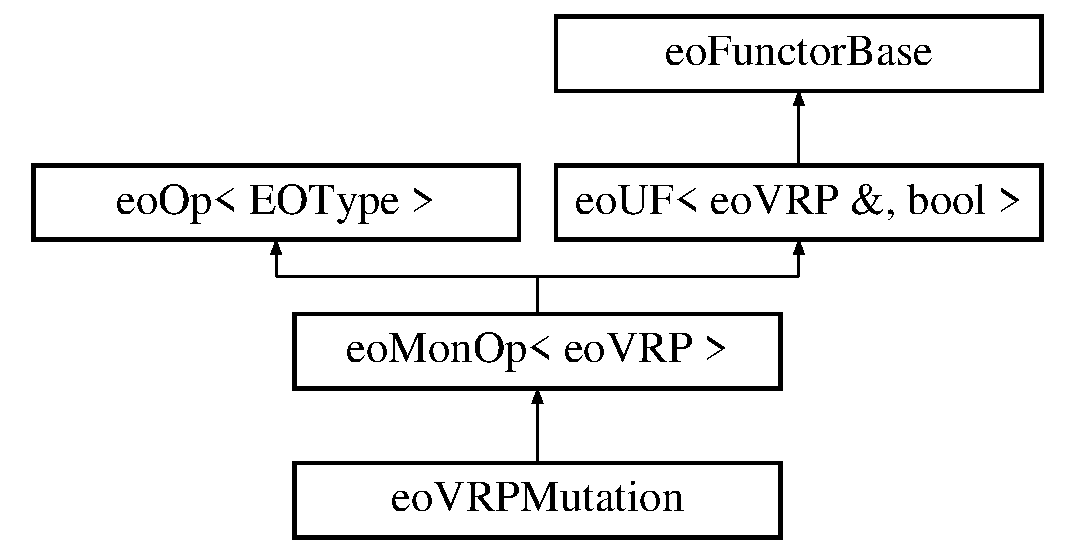
\includegraphics[height=4cm]{classeo_v_r_p_mutation}
\end{center}
\end{figure}
\subsection*{Public Member Functions}
\begin{CompactItemize}
\item 
\bf{eo\-VRPMutation} ()\label{classeo_v_r_p_mutation_419ac5c738369876de09212a844e67c3}

\begin{CompactList}\small\item\em Default constructor: nothing to do here. \item\end{CompactList}\item 
std::string \bf{class\-Name} () const 
\begin{CompactList}\small\item\em Returns a string containing the name of the class. \item\end{CompactList}\item 
bool \bf{operator()} (\bf{eo\-VRP} \&\_\-genotype)
\begin{CompactList}\small\item\em Functor operator. \item\end{CompactList}\end{CompactItemize}
\subsection*{Private Member Functions}
\begin{CompactItemize}
\item 
bool \bf{swap\-Mutation} (\bf{eo\-VRP} \&\_\-genotype)
\begin{CompactList}\small\item\em It exhanges the positions of two clients within the individual. \item\end{CompactList}\item 
bool \bf{inversion\-Mutation} (\bf{eo\-VRP} \&\_\-genotype)
\begin{CompactList}\small\item\em It selects two positions in the genotype and inverts the clients between them. \item\end{CompactList}\item 
bool \bf{insertion\-Mutation} (\bf{eo\-VRP} \&\_\-genotype)
\begin{CompactList}\small\item\em It selects and individual, erases it from its original position and inserts it somewhere else. \item\end{CompactList}\item 
bool \bf{Displacement\-Mutation} (\bf{eo\-VRP} \&\_\-genotype)
\begin{CompactList}\small\item\em It selects a set of clients, erases them from their original position and inserts them somewhere else. \item\end{CompactList}\end{CompactItemize}


\subsection{Detailed Description}
Implementation of variations of the four mutation operators for the VRP-TW defined by Tavares et al. 

These four operators should be separated in different classes and their probabilities made parameterizable. 



Definition at line 52 of file eo\-VRPMutation.h.

\subsection{Member Function Documentation}
\index{eoVRPMutation@{eo\-VRPMutation}!className@{className}}
\index{className@{className}!eoVRPMutation@{eo\-VRPMutation}}
\subsubsection{\setlength{\rightskip}{0pt plus 5cm}std::string eo\-VRPMutation::class\-Name (void) const\hspace{0.3cm}{\tt  [inline, virtual]}}\label{classeo_v_r_p_mutation_1c99e21818d6bae1cdd21b4180601d41}


Returns a string containing the name of the class. 

Used to display statistics. \begin{Desc}
\item[Returns:]The string containing the name of the class. \end{Desc}


Reimplemented from \bf{eo\-Mon\-Op$<$ eo\-VRP $>$}.

Definition at line 70 of file eo\-VRPMutation.h.\index{eoVRPMutation@{eo\-VRPMutation}!operator()@{operator()}}
\index{operator()@{operator()}!eoVRPMutation@{eo\-VRPMutation}}
\subsubsection{\setlength{\rightskip}{0pt plus 5cm}bool eo\-VRPMutation::operator() (\bf{eo\-VRP} \& {\em \_\-genotype})\hspace{0.3cm}{\tt  [inline, virtual]}}\label{classeo_v_r_p_mutation_f9fabdc8497f463add309fdace102813}


Functor operator. 

Applies one of the four mutation operators available, each of them with a predefined (hard-coded) probability. These operators should be separated in different classes and their probabilities made parameterizable to do it in a more \char`\"{}paradis\-EO\char`\"{} way. \begin{Desc}
\item[Parameters:]
\begin{description}
\item[{\em \_\-genotype}]The genotype being mutated (it will be probably modified). \end{description}
\end{Desc}
\begin{Desc}
\item[Returns:]True if the individual has been modified. False otherwise. \end{Desc}


Implements \bf{eo\-UF$<$ eo\-VRP \&, bool $>$}.

Definition at line 86 of file eo\-VRPMutation.h.

References eo\-VRP::clean\-Routes(), Displacement\-Mutation(), insertion\-Mutation(), inversion\-Mutation(), swap\-Mutation(), and eo\-Rng::uniform().\index{eoVRPMutation@{eo\-VRPMutation}!swapMutation@{swapMutation}}
\index{swapMutation@{swapMutation}!eoVRPMutation@{eo\-VRPMutation}}
\subsubsection{\setlength{\rightskip}{0pt plus 5cm}bool eo\-VRPMutation::swap\-Mutation (\bf{eo\-VRP} \& {\em \_\-genotype})\hspace{0.3cm}{\tt  [inline, private]}}\label{classeo_v_r_p_mutation_bef9736583de0b7f6e734b26483ab69d}


It exhanges the positions of two clients within the individual. 

Clients may or may not be in the same route. \begin{Desc}
\item[Parameters:]
\begin{description}
\item[{\em \_\-genotype}]The genotype being mutated (it will be probably modified). \end{description}
\end{Desc}
\begin{Desc}
\item[Returns:]True if the individual has been modified. False otherwise. \end{Desc}


Definition at line 119 of file eo\-VRPMutation.h.

References eo\-Rng::random().

Referenced by operator()().\index{eoVRPMutation@{eo\-VRPMutation}!inversionMutation@{inversionMutation}}
\index{inversionMutation@{inversionMutation}!eoVRPMutation@{eo\-VRPMutation}}
\subsubsection{\setlength{\rightskip}{0pt plus 5cm}bool eo\-VRPMutation::inversion\-Mutation (\bf{eo\-VRP} \& {\em \_\-genotype})\hspace{0.3cm}{\tt  [inline, private]}}\label{classeo_v_r_p_mutation_61cc39a190e9d070b005a7afb5e38d2a}


It selects two positions in the genotype and inverts the clients between them. 

Clients may or may not be in the same route. \begin{Desc}
\item[Parameters:]
\begin{description}
\item[{\em \_\-genotype}]The genotype being mutated (it will be probably modified). \end{description}
\end{Desc}
\begin{Desc}
\item[Returns:]True if the individual has been modified. False otherwise. \end{Desc}


Definition at line 142 of file eo\-VRPMutation.h.

References eo\-Rng::random().

Referenced by operator()().\index{eoVRPMutation@{eo\-VRPMutation}!insertionMutation@{insertionMutation}}
\index{insertionMutation@{insertionMutation}!eoVRPMutation@{eo\-VRPMutation}}
\subsubsection{\setlength{\rightskip}{0pt plus 5cm}bool eo\-VRPMutation::insertion\-Mutation (\bf{eo\-VRP} \& {\em \_\-genotype})\hspace{0.3cm}{\tt  [inline, private]}}\label{classeo_v_r_p_mutation_6ead0938bb1f8ab34c321916a6dd5b66}


It selects and individual, erases it from its original position and inserts it somewhere else. 

The insertion may or may not be within the same route. \begin{Desc}
\item[Parameters:]
\begin{description}
\item[{\em \_\-genotype}]The genotype being mutated (it will be probably modified). \end{description}
\end{Desc}
\begin{Desc}
\item[Returns:]True if the individual has been modified. False otherwise. \end{Desc}


Definition at line 170 of file eo\-VRPMutation.h.

References eo\-Rng::random().

Referenced by operator()().\index{eoVRPMutation@{eo\-VRPMutation}!DisplacementMutation@{DisplacementMutation}}
\index{DisplacementMutation@{DisplacementMutation}!eoVRPMutation@{eo\-VRPMutation}}
\subsubsection{\setlength{\rightskip}{0pt plus 5cm}bool eo\-VRPMutation::Displacement\-Mutation (\bf{eo\-VRP} \& {\em \_\-genotype})\hspace{0.3cm}{\tt  [inline, private]}}\label{classeo_v_r_p_mutation_b6b7e818085f6ba03d64f045f32356be}


It selects a set of clients, erases them from their original position and inserts them somewhere else. 

The selected set of clients may cover different routes. \begin{Desc}
\item[Parameters:]
\begin{description}
\item[{\em \_\-genotype}]The genotype being mutated (it will be probably modified). \end{description}
\end{Desc}
\begin{Desc}
\item[Returns:]True if the individual has been modified. False otherwise. \end{Desc}


Definition at line 199 of file eo\-VRPMutation.h.

References eo\-Rng::random().

Referenced by operator()().

The documentation for this class was generated from the following file:\begin{CompactItemize}
\item 
eo\-VRPMutation.h\end{CompactItemize}

\section{eo\-VRPOne\-Point\-Crossover Class Reference}
\label{classeo_v_r_p_one_point_crossover}\index{eoVRPOnePointCrossover@{eoVRPOnePointCrossover}}
Implementation of the simple One Point Crossover.  


{\tt \#include $<$eo\-VRPQuad\-Crossover.h$>$}

Inheritance diagram for eo\-VRPOne\-Point\-Crossover::\begin{figure}[H]
\begin{center}
\leavevmode
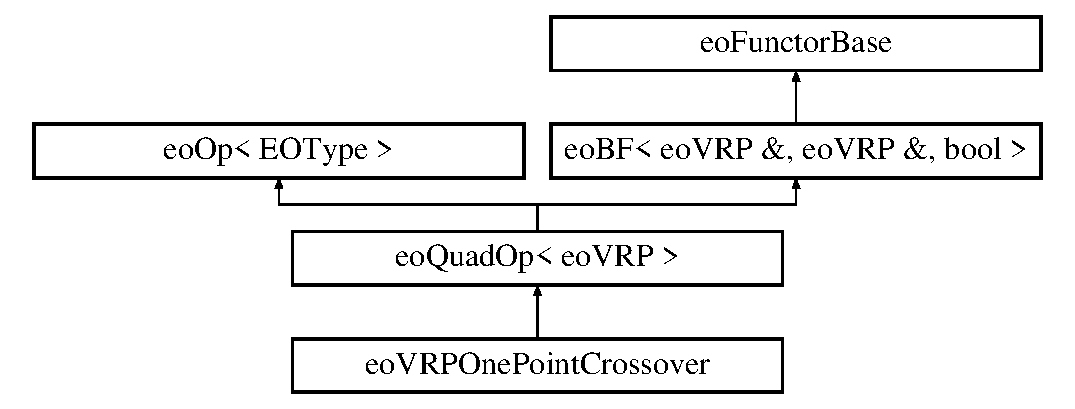
\includegraphics[height=4cm]{classeo_v_r_p_one_point_crossover}
\end{center}
\end{figure}
\subsection*{Public Member Functions}
\begin{CompactItemize}
\item 
\bf{eo\-VRPOne\-Point\-Crossover} ()\label{classeo_v_r_p_one_point_crossover_24f40efc1adb60947c5d533653bbfbe9}

\begin{CompactList}\small\item\em Deafult constructor. \item\end{CompactList}\item 
std::string \bf{class\-Name} () const 
\begin{CompactList}\small\item\em Returns a string containing the name of the class. \item\end{CompactList}\item 
bool \bf{operator()} (\bf{eo\-VRP} \&\_\-genotype1, \bf{eo\-VRP} \&\_\-genotype2)
\begin{CompactList}\small\item\em Performs a one point crossover. \item\end{CompactList}\end{CompactItemize}


\subsection{Detailed Description}
Implementation of the simple One Point Crossover. 



Definition at line 159 of file eo\-VRPQuad\-Crossover.h.

\subsection{Member Function Documentation}
\index{eoVRPOnePointCrossover@{eo\-VRPOne\-Point\-Crossover}!className@{className}}
\index{className@{className}!eoVRPOnePointCrossover@{eo\-VRPOne\-Point\-Crossover}}
\subsubsection{\setlength{\rightskip}{0pt plus 5cm}std::string eo\-VRPOne\-Point\-Crossover::class\-Name (void) const\hspace{0.3cm}{\tt  [inline, virtual]}}\label{classeo_v_r_p_one_point_crossover_a62bc52e6f36d7fae7c192173fbfd2dc}


Returns a string containing the name of the class. 

Used to display statistics. \begin{Desc}
\item[Returns:]The string containing the name of the class. \end{Desc}


Reimplemented from \bf{eo\-Quad\-Op$<$ eo\-VRP $>$}.

Definition at line 177 of file eo\-VRPQuad\-Crossover.h.\index{eoVRPOnePointCrossover@{eo\-VRPOne\-Point\-Crossover}!operator()@{operator()}}
\index{operator()@{operator()}!eoVRPOnePointCrossover@{eo\-VRPOne\-Point\-Crossover}}
\subsubsection{\setlength{\rightskip}{0pt plus 5cm}bool eo\-VRPOne\-Point\-Crossover::operator() (\bf{eo\-VRP} \& {\em \_\-genotype1}, \bf{eo\-VRP} \& {\em \_\-genotype2})\hspace{0.3cm}{\tt  [inline, virtual]}}\label{classeo_v_r_p_one_point_crossover_b930b5d9a8ee0719f675f9eea791579b}


Performs a one point crossover. 

Both parameters are the parents and the (future) children of the crossover. \begin{Desc}
\item[Parameters:]
\begin{description}
\item[{\em \_\-genotype1}]The first parent. \item[{\em \_\-genotype2}]The second parent. \end{description}
\end{Desc}
\begin{Desc}
\item[Returns:]True if any of the parents was modified. False otherwise. \end{Desc}


Implements \bf{eo\-BF$<$ eo\-VRP \&, eo\-VRP \&, bool $>$}.

Definition at line 191 of file eo\-VRPQuad\-Crossover.h.

References eo\-VRP::clean\-Routes(), and eo\-Rng::random().

The documentation for this class was generated from the following file:\begin{CompactItemize}
\item 
eo\-VRPQuad\-Crossover.h\end{CompactItemize}

\section{eo\-VRPStat Class Reference}
\label{classeo_v_r_p_stat}\index{eoVRPStat@{eoVRPStat}}
Manages the statistics of the VRP problem.  


{\tt \#include $<$eo\-VRPStat.h$>$}

Inheritance diagram for eo\-VRPStat::\begin{figure}[H]
\begin{center}
\leavevmode
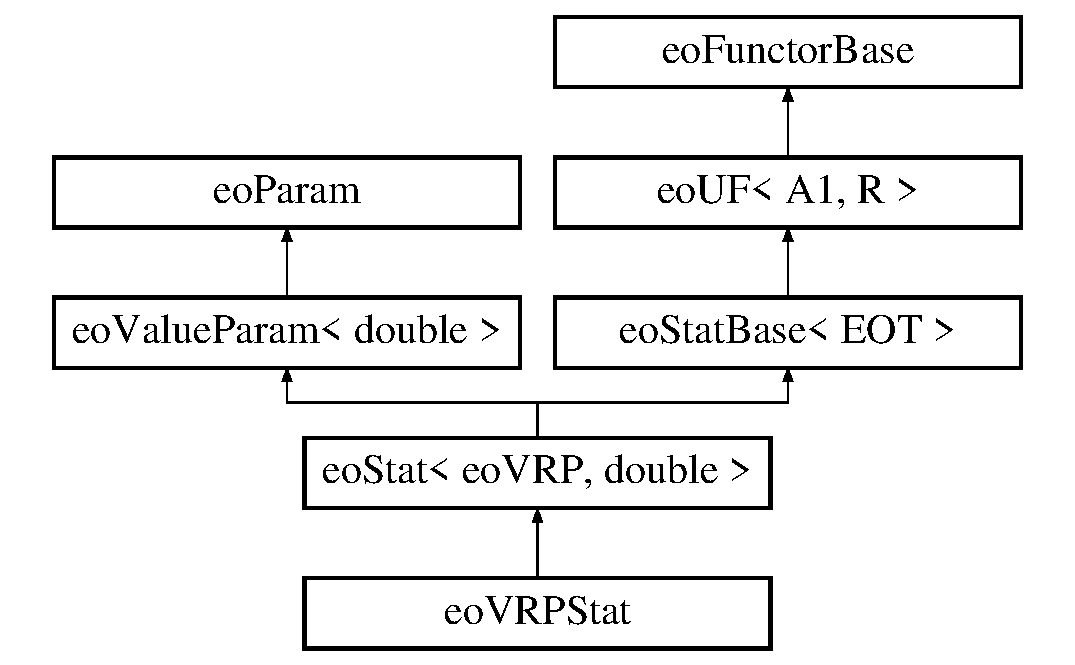
\includegraphics[height=5cm]{classeo_v_r_p_stat}
\end{center}
\end{figure}
\subsection*{Public Member Functions}
\begin{CompactItemize}
\item 
\bf{eo\-VRPStat} (std::string \_\-description=\char`\"{}eo\-VRPStat \char`\"{})
\begin{CompactList}\small\item\em Constructor: initializes variables properly. \item\end{CompactList}\item 
void \bf{operator()} (const \bf{eo\-Pop}$<$ \bf{eo\-VRP} $>$ \&\_\-pop)
\begin{CompactList}\small\item\em Gets statistics from a population. \item\end{CompactList}\item 
virtual std::string \bf{class\-Name} (void) const 
\begin{CompactList}\small\item\em Returns a string containing the name of the class. \item\end{CompactList}\end{CompactItemize}


\subsection{Detailed Description}
Manages the statistics of the VRP problem. 



Definition at line 47 of file eo\-VRPStat.h.

\subsection{Constructor \& Destructor Documentation}
\index{eoVRPStat@{eo\-VRPStat}!eoVRPStat@{eoVRPStat}}
\index{eoVRPStat@{eoVRPStat}!eoVRPStat@{eo\-VRPStat}}
\subsubsection{\setlength{\rightskip}{0pt plus 5cm}eo\-VRPStat::eo\-VRPStat (std::string {\em \_\-description} = {\tt \char`\"{}eoVRPStat~\char`\"{}})\hspace{0.3cm}{\tt  [inline]}}\label{classeo_v_r_p_stat_a326e09d7efebb4c572ea51ae517e058}


Constructor: initializes variables properly. 

\begin{Desc}
\item[Parameters:]
\begin{description}
\item[{\em \_\-description}]A string identifying the class. \end{description}
\end{Desc}


Definition at line 56 of file eo\-VRPStat.h.

\subsection{Member Function Documentation}
\index{eoVRPStat@{eo\-VRPStat}!operator()@{operator()}}
\index{operator()@{operator()}!eoVRPStat@{eo\-VRPStat}}
\subsubsection{\setlength{\rightskip}{0pt plus 5cm}void eo\-VRPStat::operator() (const \bf{eo\-Pop}$<$ \bf{eo\-VRP} $>$ \& {\em \_\-pop})\hspace{0.3cm}{\tt  [inline]}}\label{classeo_v_r_p_stat_5e773fab9c82e0a06d075af4be265d1e}


Gets statistics from a population. 

\begin{Desc}
\item[Parameters:]
\begin{description}
\item[{\em \_\-pop}]The population that will be analyzed. \end{description}
\end{Desc}


Definition at line 66 of file eo\-VRPStat.h.

References eo\-Value\-Param$<$ T $>$::value().\index{eoVRPStat@{eo\-VRPStat}!className@{className}}
\index{className@{className}!eoVRPStat@{eo\-VRPStat}}
\subsubsection{\setlength{\rightskip}{0pt plus 5cm}virtual std::string eo\-VRPStat::class\-Name (void) const\hspace{0.3cm}{\tt  [inline, virtual]}}\label{classeo_v_r_p_stat_61d9ece1bde19f4cd997c3aba075d8e7}


Returns a string containing the name of the class. 

Used to display statistics. \begin{Desc}
\item[Returns:]The string containing the name of the class. \end{Desc}


Reimplemented from \bf{eo\-Stat$<$ eo\-VRP, double $>$}.

Definition at line 79 of file eo\-VRPStat.h.

The documentation for this class was generated from the following file:\begin{CompactItemize}
\item 
eo\-VRPStat.h\end{CompactItemize}

\printindex
\end{document}
